
%% V0.1
%% 2017/06/02
%% by Xi Huang

\documentclass[10pt,journal,compsoc]{IEEEtran}

% *** CITATION PACKAGES ***
%
\ifCLASSOPTIONcompsoc
  % IEEE Computer Society needs nocompress option
  % requires cite.sty v4.0 or later (November 2003)
  \usepackage[nocompress]{cite}
\else
  % normal IEEE
  \usepackage{cite}
\fi

\usepackage{graphicx}
\graphicspath{{./figures/}}
\DeclareGraphicsExtensions{.eps}

\usepackage{amsmath}
\usepackage{amsfonts}
\usepackage{color}
\usepackage{amssymb}
\usepackage{algorithm}
\usepackage{algorithmic}
\usepackage{array}
\usepackage{url}

\usepackage{subfigure}

\ifCLASSOPTIONcompsoc
  \usepackage[caption=false,font=normalsize,labelfont=sf,textfont=sf]{subfig}
\else
  \usepackage[caption=false,font=footnotesize]{subfig}
\fi

% Define new command for theorem proof
\newtheorem{lemma}{Lemma}
\newtheorem{definition}{Definition}
\newtheorem{theorem}{Theorem}
\newtheorem{proof}{Proof}
\newtheorem{proposition}{Proposition}
\newtheorem{corollary}{Corollary}
\newtheorem{remark}{Remark}
% End of defining for theorem proof commands

% *** Do not adjust lengths that control margins, column widths, etc. ***
% *** Do not use packages that alter fonts (such as pslatex).         ***
% There should be no need to do such things with IEEEtran.cls V1.6 and later.
% (Unless specifically asked to do so by the journal or conference you plan
% to submit to, of course. )


% correct bad hyphenation here
\hyphenation{net-works}


\begin{document}
%
% paper title
% Titles are generally capitalized except for words such as a, an, and, as,
% at, but, by, for, in, nor, of, on, or, the, to and up, which are usually
% not capitalized unless they are the first or last word of the title.
% Linebreaks \\ can be used within to get better formatting as desired.
% Do not put math or special symbols in the title.
\title{Dynamic Switch-Controller Association and Control Devolution for SDN Systems}
%
%
% author names and IEEE memberships
% note positions of commas and nonbreaking spaces ( ~ ) LaTeX will not break
% a structure at a ~ so this keeps an author's name from being broken across
% two lines.
% use \thanks{} to gain access to the first footnote area
% a separate \thanks must be used for each paragraph as LaTeX2e's \thanks
% was not built to handle multiple paragraphs
%
%
%\IEEEcompsocitemizethanks is a special \thanks that produces the bulleted
% lists the Computer Society journals use for "first footnote" author
% affiliations. Use \IEEEcompsocthanksitem which works much like \item
% for each affiliation group. When not in compsoc mode,
% \IEEEcompsocitemizethanks becomes like \thanks and
% \IEEEcompsocthanksitem becomes a line break with idention. This
% facilitates dual compilation, although admittedly the differences in the
% desired content of \author between the different types of papers makes a
% one-size-fits-all approach a daunting prospect. For instance, compsoc 
% journal papers have the author affiliations above the "Manuscript
% received ..."  text while in non-compsoc journals this is reversed. Sigh.

%\author{Michael~Shell,~\IEEEmembership{Member,~IEEE,}
%        John~Doe,~\IEEEmembership{Fellow,~OSA,}
%        and~Jane~Doe,~\IEEEmembership{Life~Fellow,~IEEE}% <-this % stops a space
\author{\IEEEauthorblockN{Xi Huang$^{1}$, Simeng Bian$^{1}$, Ziyu Shao$^{1}$, Hong Xu$^{2}$}
\IEEEauthorblockA{\\$^{1}$School of Information Science and Technology, ShanghaiTech University\\
 $^{2}$ NetX Lab @ City University of Hong Kong \\
 Email: \{huangxi,biansm,shaozy\}@shanghaitech.edu.cn, henry.xu@cityu.edu.hk}}
%\IEEEcompsocitemizethanks{\IEEEcompsocthanksitem M. Shell was with the Department
%of Electrical and Computer Engineering, Georgia Institute of Technology, Atlanta,
%GA, 30332.\protect\\
%% note need leading \protect in front of \\ to get a newline within \thanks as
%% \\ is fragile and will error, could use \hfil\break instead.
%E-mail: see http://www.michaelshell.org/contact.html
%\IEEEcompsocthanksitem J. Doe and J. Doe are with Anonymous University.}% <-this % stops an unwanted space
%\thanks{Manuscript received April 19, 2005; revised August 26, 2015.}

% note the % following the last \IEEEmembership and also \thanks - 
% these prevent an unwanted space from occurring between the last author name
% and the end of the author line. i.e., if you had this:
% 
% \author{....lastname \thanks{...} \thanks{...} }
%                     ^------------^------------^----Do not want these spaces!
%
% a space would be appended to the last name and could cause every name on that
% line to be shifted left slightly. This is one of those "LaTeX things". For
% instance, "\textbf{A} \textbf{B}" will typeset as "A B" not "AB". To get
% "AB" then you have to do: "\textbf{A}\textbf{B}"
% \thanks is no different in this regard, so shield the last } of each \thanks
% that ends a line with a % and do not let a space in before the next \thanks.
% Spaces after \IEEEmembership other than the last one are OK (and needed) as
% you are supposed to have spaces between the names. For what it is worth,
% this is a minor point as most people would not even notice if the said evil
% space somehow managed to creep in.



% The paper headers
\markboth{IEEE TRANSACTIONS ON SERVICES COMPUTING,~Vol.~XX, No.~X, August~2017}%
{Shell \MakeLowercase{\textit{et al.}}: Bare Demo of IEEEtran.cls for Computer Society Journals}
% The only time the second header will appear is for the odd numbered pages
% after the title page when using the twoside option.
% 
% *** Note that you probably will NOT want to include the author's ***
% *** name in the headers of peer review papers.                   ***
% You can use \ifCLASSOPTIONpeerreview for conditional compilation here if
% you desire.



% The publisher's ID mark at the bottom of the page is less important with
% Computer Society journal papers as those publications place the marks
% outside of the main text columns and, therefore, unlike regular IEEE
% journals, the available text space is not reduced by their presence.
% If you want to put a publisher's ID mark on the page you can do it like
% this:
%\IEEEpubid{0000--0000/00\$00.00~\copyright~2015 IEEE}
% or like this to get the Computer Society new two part style.
%\IEEEpubid{\makebox[\columnwidth]{\hfill 0000--0000/00/\$00.00~\copyright~2015 IEEE}%
%\hspace{\columnsep}\makebox[\columnwidth]{Published by the IEEE Computer Society\hfill}}
% Remember, if you use this you must call \IEEEpubidadjcol in the second
% column for its text to clear the IEEEpubid mark (Computer Society jorunal
% papers don't need this extra clearance.)



% use for special paper notices
%\IEEEspecialpapernotice{(Invited Paper)}


\IEEEtitleabstractindextext{%
\begin{abstract}

In software-defined networking (SDN), as data plane scale expands, scalability and reliability of the control plane have become major concerns. To mitigate such concerns, two kinds of solutions have been proposed separately. One is multi-controller architecture, i.e., a logically centralized control plane with physically distributed controllers. The other is control devolution, i.e., delegating control of some flows back to switches. Most of existing solutions adopt either static switch-controller association or static devolution, which may not adapt well to the traffic variation, leading to high communication costs between switches and controller, and high computation costs of switches.  
In this paper, we propose a novel scheme to jointly consider both solutions, i.e., we dynamically associate switches with controllers and dynamically devolve control of flows to switches. Our scheme is an efficient online algorithm that does not need the statistics of traffic flows. By adjusting some parameter $V$, we can make a trade-off between costs and queue backlogs. Theoretical analysis and extensive simulations show that our scheme yields much lower costs and latency compared to static schemes, and balanced loads among controllers. 

\end{abstract}

% Note that keywords are not normally used for peerreview papers.
\begin{IEEEkeywords}
Cloud computing, .
\end{IEEEkeywords}}


% make the title area
\maketitle


% To allow for easy dual compilation without having to reenter the
% abstract/keywords data, the \IEEEtitleabstractindextext text will
% not be used in maketitle, but will appear (i.e., to be "transported")
% here as \IEEEdisplaynontitleabstractindextext when the compsoc 
% or transmag modes are not selected <OR> if conference mode is selected 
% - because all conference papers position the abstract like regular
% papers do.
\IEEEdisplaynontitleabstractindextext
% \IEEEdisplaynontitleabstractindextext has no effect when using
% compsoc or transmag under a non-conference mode.



% For peer review papers, you can put extra information on the cover
% page as needed:
% \ifCLASSOPTIONpeerreview
% \begin{center} \bfseries EDICS Category: 3-BBND \end{center}
% \fi
%
% For peerreview papers, this IEEEtran command inserts a page break and
% creates the second title. It will be ignored for other modes.
\IEEEpeerreviewmaketitle



\IEEEraisesectionheading{\section{Introduction}\label{sec:introduction}}
\IEEEPARstart{S}{oftware-defined networking} (SDN) holds great promises to improve network performance and management. The key idea of SDN is to decouple the control plane from the data plane \cite{mckeown2008openflow}. Data plane can focus on performing basic functionalities such as packet forwarding at high speed, while the logically centralized control plane manages the network. Usually, switches at data plane send request to control plane for processing some flow events, e.g. flow-install events.

The control plane is a potential bottleneck of SDN in terms of scalability and reliability. As the data plane expands, control plane may not be able to process the increasing number of requests if implemented with a single controller, resulting unacceptable latency to flow setup. Reliability is also an issue since a single controller is a single point of failure , resulting in disastrous break-down of the control plane and the network. 

Existing proposals to address such problems fall broadly into two categories. One is to implement the control plane as a distributed system with multiple controllers \cite{koponen2010onix} \cite{tootoonchian2010hyperflow}. Each switch then associate with certain controller for fault-tolerance and load balancing \cite{levin2012logically} \cite{dixit2013towards}\cite{krishnamurthy2014pratyaastha}\cite{wang2016dynamic}. The other is to devolve partial loads of request processing from controllers to switches \cite{curtis2011devoflow} \cite{hassas2012kandoo}  \cite{zheng2015lazyctrl}, reducing the work load of controllers.

For switch-controller association, the first category of solution, initial design choice is to make a static switch-controller association \cite{koponen2010onix} \cite{tootoonchian2010hyperflow}. However, such static association may result in overloading of controllers and increasing flow setup latency due to its inflexibility to handle traffic variations. An elastic distributed controller architecture is proposed in \cite{dixit2013towards}, with an efficient protocol to migrate switches across controllers. However, it remains open to determine the switch-controller association. Then \cite{krishnamurthy2014pratyaastha} took a step further by formulating the switch-association problem as a deterministic optimization problem, i.e., an integer linear problem with prohibitively high computational complexity. A local search algorithm was proposed to find suboptimal associations within a given time limit (e.g., 30 seconds). In \cite{wang2016dynamic}, the controller is assumed to be modeled as M/M/1 queue (Poisson arrival and exponential service). Under such assumption, the switch-association problem with steady-state objective function was formulated as a many-to-one stable matching problem with transfers. Then a novel two-phase algorithm was proposed to connect stable matching with utility-based game theoretic solutions, i.e., coalition formation game with Nash stable solutions.  

For control devolution, the second category of solution, initial design choice is to make a static devolution for certain functions and certain flows \cite{curtis2011devoflow} \cite{hassas2012kandoo}  \cite{zheng2015lazyctrl}. It remains open for dynamic devolution with respect to traffic variations.  

Then several interesting questions are raised and answers to such questions will definitely shape our design for SDN networks:
\begin{itemize}
  \item[i.] Instead of deterministic switch-controller association with infrequent re-association \cite{krishnamurthy2014pratyaastha} \cite{wang2016dynamic}, can we directly perform dynamic switch-controller association with respect to the traffic variation? What is the benefit that we can obtain from a fine-grained control at the request level?
  \item[ii.] How to perform dynamic devolution?
  \item[iii.] How to make a trade-off between dynamic switch-controller association and dynamic control devolution?   
\end{itemize}

In this paper, we consider a general SDN network with traffic variations, resulting variations of requests to handle with flow events. We assume each request can be either processed at switch (incurs computation costs) or be uploaded to certain controllers (incurs communication costs) \footnote{The scenario that some requests can only be processed by controller is a straightforward extension of our model.}. We aim at reducing the computational cost by control devolution at data plane, the communication cost by switch-user association between data plane and control plane, and the response time experienced by switches, which is mainly caused by queueing delay on controllers. Under such settings, we provide a new perspective and a novel scheme to answer those questions. Our key results and contributions are summarized as follows:

 \begin{enumerate}
  \item[i.] \textit{Problem Formulation}: According to the best of our knowledge, this paper is the first to study the joint optimization problem of dynamic switch-controller association and dynamic control devolution.   
  \item[ii.] \textit{Finer Granularity Control}: According to the best of our knowledge, this paper is the first to perform the control decisions at the granularity of request-level. Note that request-level information such as time-varying queue backlog sizes and number of request arrivals presents the actual time-varying state of data plane. Hence it'd help for more accurate decision making of dynamic association and dynamic devolution when compared to coarse-grained control. 
  \item[iii.] \textit{Online Algorithm Design}: We formulate a stochastic network optimization problem, aiming at minimizing the long-term average sum of communication cost and computational cost, while keeping time-average queue backlogs of both switches and controllers small \footnote{By applying \emph{Little's law}, small queue backlog implies small queueing delay or short response time.}. By employing Lyapunov drift technique \cite{neely2010stochastic} and exploiting sub-problem’s structure, we develop an efficient greedy algorithm to achieve optimality asymptotically. Our algorithm is online, which means it does not need the statistics of traffic workloads and does not need the prior assumption of traffic distribution. 
  \item[iv.] \textit{Algorithm Analysis}: We show that our algorithm yields a tunable trade-off between $O(1/V)$ deviation from minimum long-term average sum of communication cost and computational cost and $O(V)$ bound for average queue backlogs. We also find that the positive parameter $V$ determines the switches' willingness of uploading requests to controllers, i.e., performing switch-controller association. 
  \item[v.] \textit{Simulation}: We conduct large-scale trace-driven simulations to evaluate the performance of our algorithm within two widely adopted data center networking topologies, i.e., Canonical 3-Tiered topology and Fat-tree topology. Simulation results verify the effectiveness and the trade-off of our algorithm. In addition, in the extreme case that without control devolution, we compare our dynamic association scheme with other association schemes including Static, Random, and JSQ (join the shortest queue). Simulation results verify the advantages of our schemes. 
 \end{enumerate}
 
We organize the rest of paper as follows. We present the basic idea and formulation in Section 2. Then we show our algorithm design and corresponding performance analysis in Section 3. In Section 4, we present simulation results. We conclude this paper in Section 5. 

\section{Problem Formulation}

In this section, we first provide a motivating example for the dynamic switch-controller association and dynamic control devolution. Then we introduce the system model and formulate the problem.

\subsection{Motivating Example}

The example of dynamic association and devolution is shown in Fig. \ref{fig_sim}.

\begin{figure}[!t]
\centering
 {
 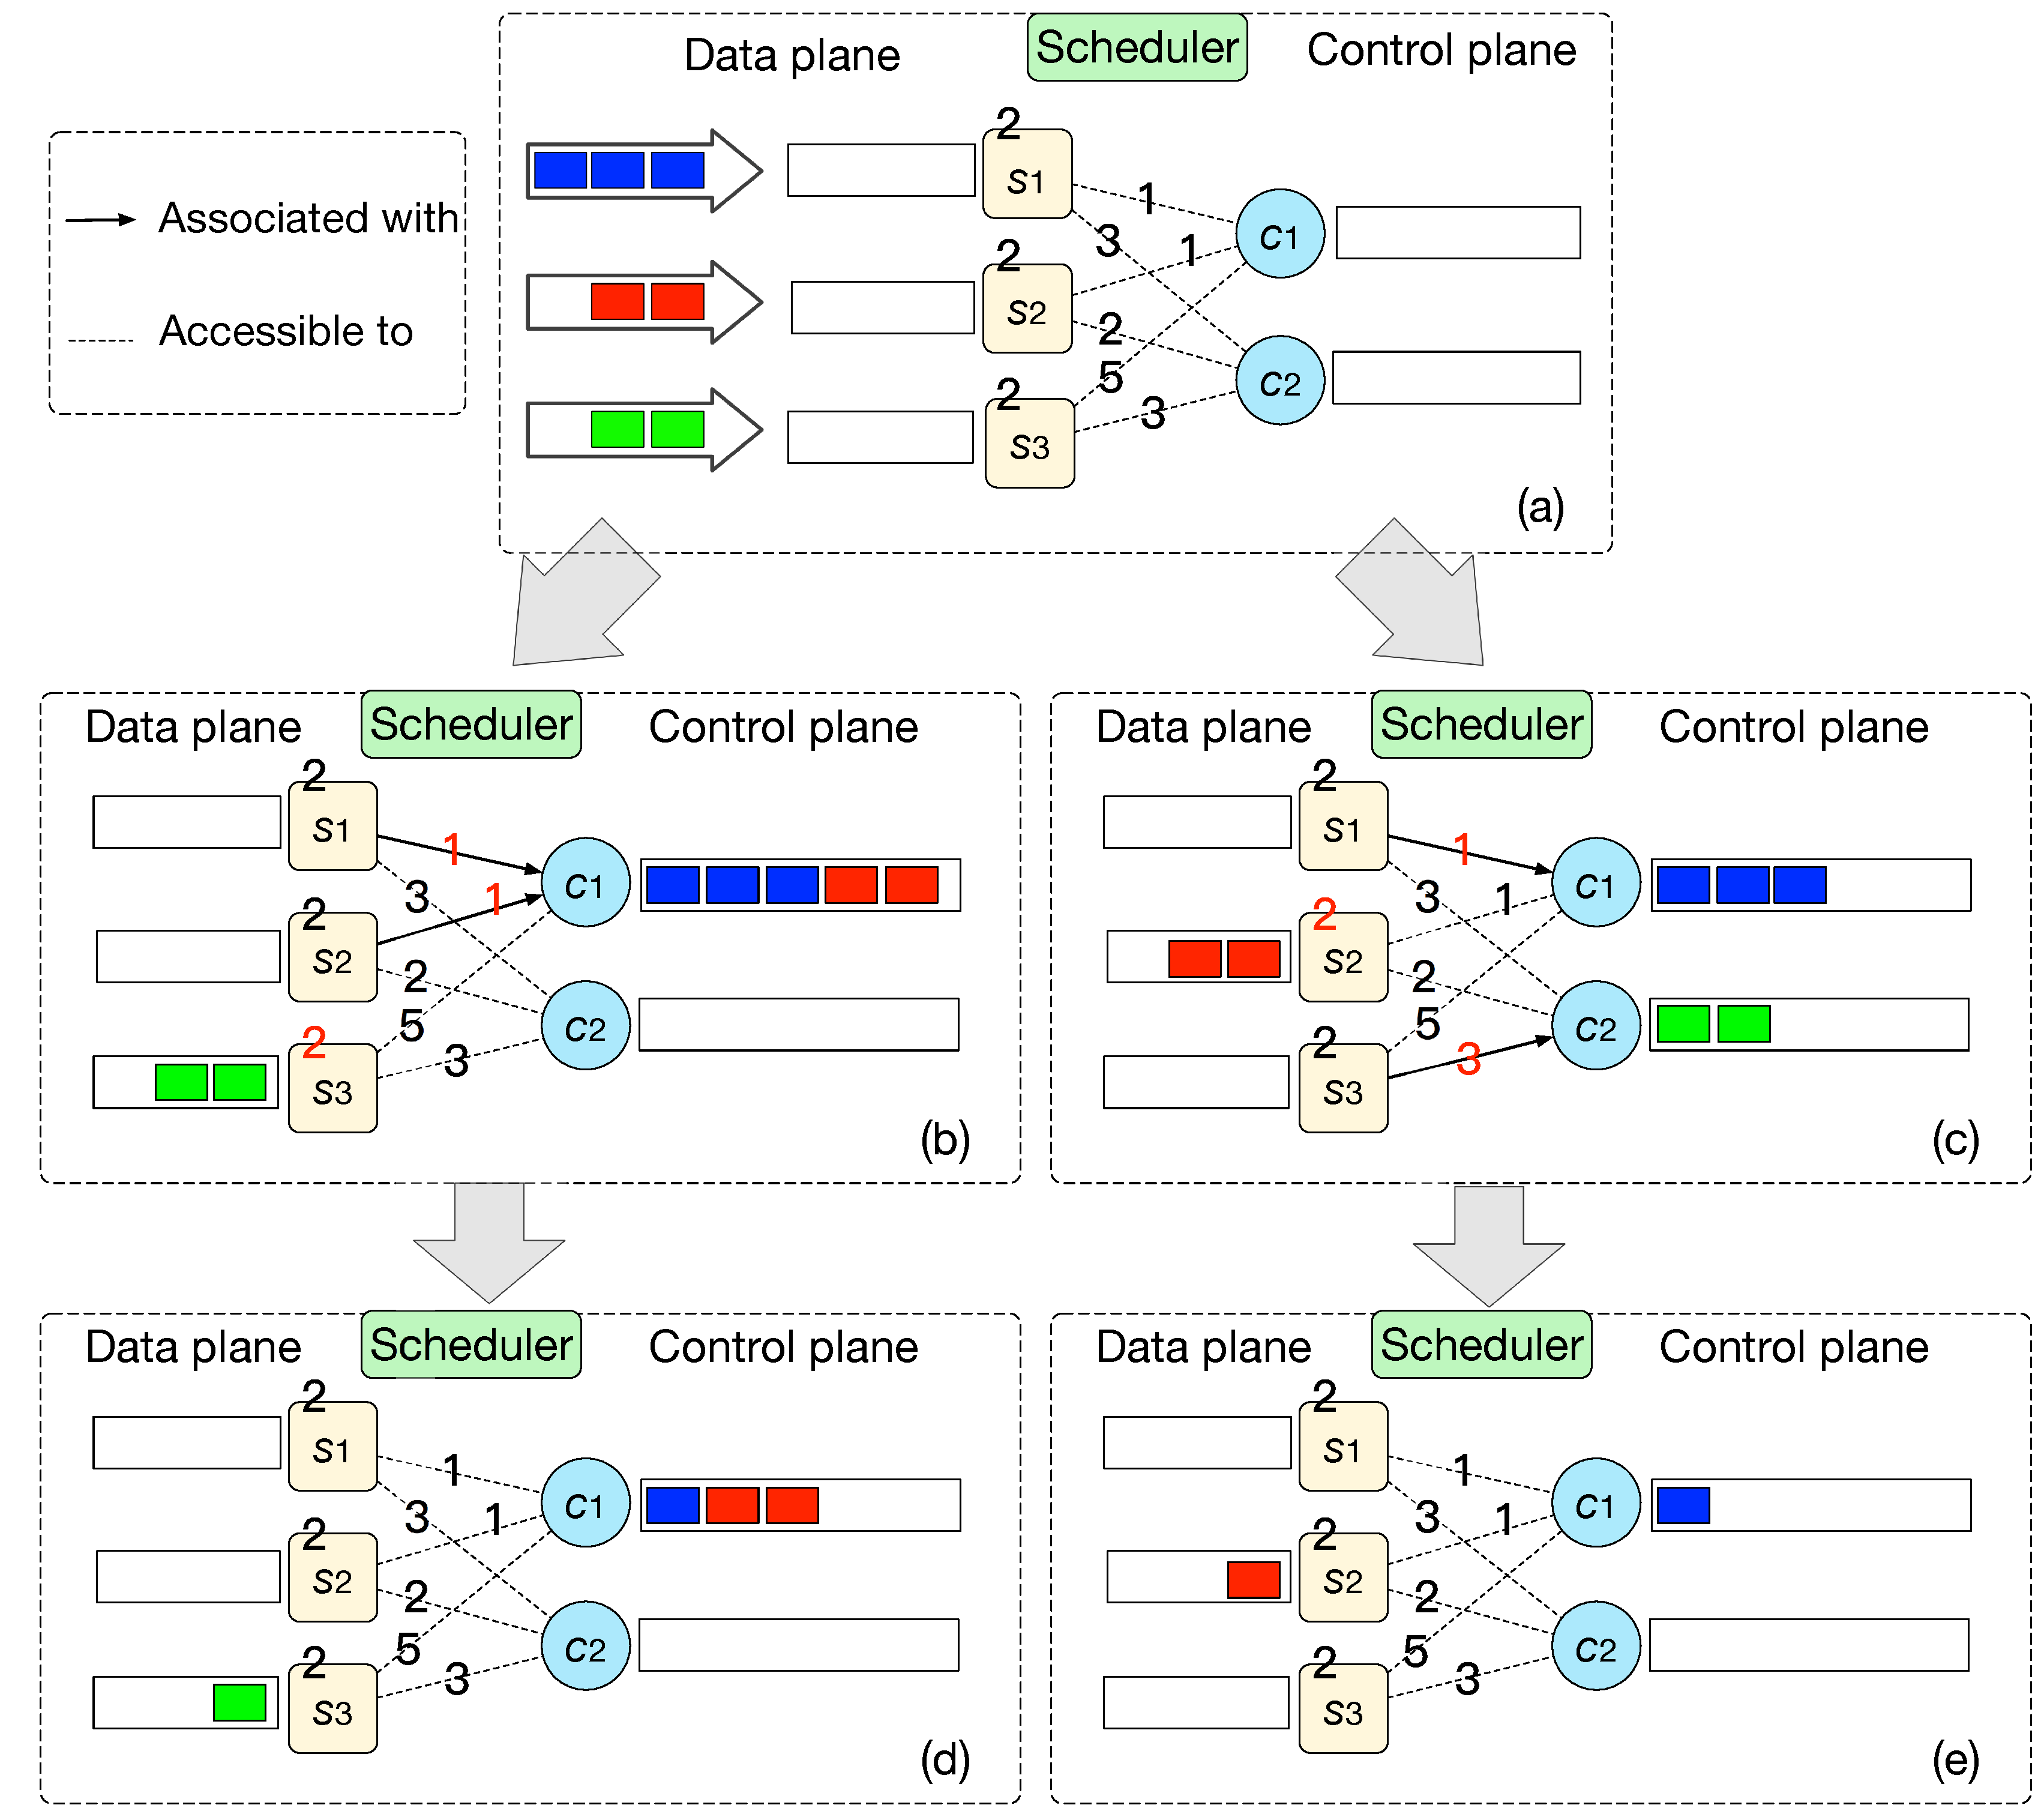
\includegraphics[width=1.0\columnwidth]{demo.eps}
 }
 \caption{An example that shows the request-level scheduling process. 
There are $3$ switches$(s_1,s_2,s_3)$, $2$ controllers$(c_1,c_2)$, and $1$ global scheduler. 
Each switch or controller maintains a queue that buffers requests. 
During each time slot, each switch can decide to store and process its requests locally or to upload requests to some controller at each time slot. Each controller can serve $2$ requests while each switch can serve only $1$ request. There is a communication cost per request if switches upload requests to controllers, and a computational cost ($2$ per request on each switch) from local processing by switches themselves. At the beginning of time slot $t$, $s_1$, $s_2$, and $s_3$ generates $3$, $2$, and $2$ requests, respectively. The scheduler then collects system dynamics and decides a switch-controller association (could be (b) or (c)), aiming at minimizing the sum of communication cost (could be the number of hops, RTTs, etc.) and computational cost, as well as maintaining small queue backlog size. Each switch chooses to either locally process its requests or send them to controllers according to the scheduling decision.}
 \label{fig_sim}
\end{figure}

First, we focus on the behavior of $s_3$. In Fig. \ref{fig_sim} (b), $s_3$ chooses to process its requests locally,  and that incurs a computational cost of 2 per request. In Fig. \ref{fig_sim} (c), $s_3$ decides to upload requests to $c_2$ and that incurs a communication cost of 3 per request. Although the computational cost is less than communication cost, the decision of locally processing leaves one request not processed yet at the end of the time slot. Hence, it is not necessarily a smart decision for a switch to perform control devolution when its computational cost is lower than its communication cost. Instead, the scheduler should jointly decide control devolution and switch-controller association at the same time.

Second, we focus on the behavior of associations. Fig. \ref{fig_sim} (b) and (c) show two different associations. Fig. \ref{fig_sim} (b) shows the switch-controller association with $(s_1, c_1)$ and $(s_2, c_1)$ ($s_3$ processes requests locally), denoted by $X_1$. $X_1$ incurs the total cost of communication and computation by $9$ but results in uneven queue backlogs, leaving four requests unfinished after time slot $t$. Fig. \ref{fig_sim} (c) shows another association with $(s_1, c_1)$ and $(s_3, c_2)$ ($s_2$ processes requests locally), denoted by $X_2$. $X_2$ incurs the total cost by $13$ but does better in balancing queue backlogs. Thus there is a non-trivial trade-off between minimizing the total cost of communication and computation and maintaining small queue backlogs on each controller.

\subsection{Problem Formulation}

We consider a time slotted network system, indexed by $\{0,1,\,2,\,\dots\}$. Its control plane comprises a set $\mathcal{C}$ of physically distributed controllers, while its data plane consists of a set of switches $\mathcal{S}$. 
%We use ${C}$ and ${S}$ to denote the size of $\mathcal{C}$ and $\mathcal{S}$, respectively. 
Each switch $i \in \mathcal{S}$ keeps a queue backlog of size $Q^s_i(t)$ for locally processing requests, while each controller $j \in \mathcal{C}$ maintains a queue backlog $Q^c_j(t)$ that buffers requests from data plane. We denote $[ Q^c_1(t),\,\dots,\,Q^c_{|\mathcal{C}|}(t) ]$ as $\mathbf{Q}^c(t)$ and $[ Q^s_1(t),\,\dots,\,Q^s_{|\mathcal{S}|}(t) ]$ as $\mathbf{Q}^s(t)$. We use $\mathbf{Q}(t)$ to denote $[\mathbf{Q}^s(t), \mathbf{Q}^c(t)]$.

At the beginning of time slot $t$, each switch $i \in \mathcal{S}$ generates some amounts $0 \le A_i(t) \le a_{max}$ of requests. Then each switch could choose to process its requests either locally or by sending to its associated controller. We assume that each switch $i \in \mathcal{S}$ has a service rate $0 \le U_i(t) \le u_{max}$ to process the devoluted requests, while each controller $j \in \mathcal{C}$ has an available service rate $0 \le B_j(t) \le b_{max}$. We denote $[ A_1(t),\,\dots,\,A_{|\mathcal{S}|}(t) ]$ as $\mathbf{A}(t)$, $[ B_1(t),\,\dots,\,B_{|\mathcal{C}|}(t) ]$ as $\mathbf{B}(t)$, and $\left[ U_1(t),\,\dots,\,U_{|\mathcal{S}|}(t) \right]$ as $\mathbf{U}(t)$. For $i \in \mathcal{S}$ and $j \in \mathcal{C}$, we assume that all $A_i(t)$, $B_j(t)$, and $U_i(t)$ are i.i.d.; besides, their first and second raw moments are all finite.

%$E\{A_i(t)\} = \lambda_i < \infty$, $E\{B_j(t)\} = \theta_j < \infty$, and $E\{U_i(t)\} = u_i < \infty$; $E\{\left(A_i(t)\right)^2\}$, $E\{\left(B_j(t)\right)^2\}$, and $E\{ \left(U_i(t)\right)^2 \}$ are finite.

Then the scheduler collects system dynamics information $\left( \mathbf{A}(t),\,\mathbf{B}(t), \mathbf{Q}(t) \right)$ during current time slot and makes a scheduling decision, denoted by an association matrix $\mathbf{X}(t) \in \{0,\,1\}^{|\mathcal{S}| \times |\mathcal{C}|}$. Here $\mathbf{X}(t)_{i,j} = 1$ if switch $i$ will be associated with controller $j$ during current time slot and $0$ otherwise. An association is feasible if it guarantees that each switch is associated with at most one controller during each time slot. We denote the set of feasible associations as $\mathcal{A}$,
\begin{equation}\label{constraint set}
	\begin{array}{c}
		\displaystyle	\mathcal{A} \triangleq \left\{ \mathbf{X} \in \{0,1\}^{|\mathcal{S}| \times |\mathcal{C}|}\,|\,\sum_{j \in \mathcal{C}} \mathbf{X}_{i,j} \, \le \, 1 \text{ for } i \in \mathcal{S} \right\}
	\end{array}
\end{equation}

According to the scheduling decision, each switch $i$ sends its request to controller $j$ if $\mathbf{X}_{i,j} = 1$. However, if $\sum_{j \in \mathcal{C}} \mathbf{X}_{i,j} = 0$, switch $i$ appends its requests to local queue backlog. Then both switches and controllers serve as many requests in their queues as they could\footnote{Note that we do not fix the serving principle, which can be \emph{FIFO}, \emph{LIFO}, etc. But in our simulation, we use \emph{FIFO}.}. 
As a result, the update equation for $Q^s_i(t)$ at switch $i$ is 
\begin{equation}\label{ueq for s}
\begin{array}{c}
	\displaystyle Q^s_i(t+1) = \left[ Q^s_i(t) + \left( 1 - \sum_{j \in \mathcal{C}} \mathbf{X}_{i,j}(t) \right) {A}_{i}(t) - U_i(t)\right]^{+}
\end{array}
\end{equation}
and the update equation for $Q^c_j(t)$ at controller $j$ is given by
\begin{equation}\label{ueq for c}
\begin{array}{c}
	\displaystyle Q^c_j(t+1) = \left[ Q^c_j(t) + \sum_{i \in \mathcal{S}} \mathbf{X}_{i,j}(t)\cdot {A}_{i}(t) - B_j(t)\right]^{+}
\end{array}
\end{equation}
where $\left[\,x\,\right]^{+} = \max(x,0)$. 

Having covered the necessary notations and queueing dynamics, we switch to the objective and constraints of our problem. 

\subsubsection{Time-Average Communication Cost}

We define the communication cost between switch $i$ and controller $j$ as $W_{i,j}$ \footnote{The communication cost can be the number of hops or round trip times (RTT).}. Accordingly, we have a communication cost matrix $\mathbf{W}=\{W_{i,j}\}$. Fixing some association $\mathbf{X} \in \mathcal{A}$, the communication cost within one time slot is
\begin{equation}\label{def-commcost}
	\begin{array}{cl}
		\displaystyle f_{\mathbf{X}}(t) = \hat{f}(\mathbf{X}, \mathbf{A}(t)) \triangleq \sum_{j \in \mathcal{C}} \sum_{i \in \mathcal{S}} W_{i,j} \cdot \mathbf{X}_{i,j} \cdot A_i(t)
	\end{array}
\end{equation}
where we can view $W_{i,j}$ as the price of transmitting one request from switch $i$ to controller $j$. Then, given a series of associations $\{ \mathbf{X}_{0}, \mathbf{X}_{1}, \dots, \mathbf{X}_{t-1} \}$, the time-average expectation of communication cost is shown as follows
\begin{equation}\label{avg-commcost}
	\begin{array}{c}
		\displaystyle \bar{f}(t) \triangleq \frac{1}{t} \sum_{\tau = 0 }^{t - 1} E\left\{f_{\mathbf{X}_{\tau}}(\tau)\right\}
	\end{array}
\end{equation}

\subsubsection{Time-average Computational Cost}

There is a computational cost $\alpha_i$ for each devoluted request to $i$ when switch $i$ appends its requests to its local queue backlog for processing. Given some association $\mathbf{X} \in \mathcal{A}$, we define the one-time-slot computational cost as
\begin{equation}\label{def-offload}
	\begin{array}{cl}
		\displaystyle g_{\mathbf{X}}(t) = \hat{g}(\mathbf{X}, \mathbf{A}(t)) \triangleq \sum_{i \in \mathcal{S}} 
		\alpha_i \cdot \left( 1 - \sum_{j \in \mathcal{C}}  \mathbf{X}_{i,j} \right) \cdot A_i(t)
	\end{array}
\end{equation}
Given a series of associations $\{ \mathbf{X}_{0}, \mathbf{X}_{1}, \dots, \mathbf{X}_{t-1} \}$, the time-average expectation of computational cost is
\begin{equation}\label{avg-offload}
	\begin{array}{c}
		\displaystyle \bar{g}(t) \triangleq \frac{1}{t} \sum_{\tau = 0 }^{t - 1} E\left\{g_{\mathbf{X}_{\tau}}(\tau)\right\}
	\end{array}
\end{equation}

\subsubsection{Queueing Stability}

In this paper, we say that a queueing process $\left\{{Q}(t)\right\}$ is stable, if the following condition holds:
\begin{equation}
	\begin{array}{c}
		\displaystyle \lim_{t \to \infty} \frac{1}{t} \sum_{\tau=0}^{t-1} E\left\{Q(\tau)\right\} < \infty \\ 
	\end{array}
\end{equation}

Accordingly, for each switch $s \in \mathcal{S}$, the queueing process $\left\{ \mathbf{Q}^s(t) \right\}$ is stable if
\begin{equation}\label{stabilty2}
	\begin{array}{c}
		\displaystyle \lim_{t \to \infty} \frac{1}{t} \sum_{\tau=0}^{t-1} \sum_{i \in \mathcal{S}} E\left\{Q^s_i(\tau)\right\} < \infty
	\end{array}
\end{equation}

Likewise, for each controller $c \in \mathcal{C}$, the queueing process $\left\{ \mathbf{Q}^c(t) \right\}$ is stable if
\begin{equation}\label{stabilty1}
	\begin{array}{c}
		\displaystyle \lim_{t \to \infty} \frac{1}{t} \sum_{\tau=0}^{t-1} \sum_{j \in \mathcal{C}} E\left\{Q^c_j(\tau)\right\} < \infty
	\end{array}
\end{equation}

Queueing stability implies that both switches and controllers would process buffered requests timely, so that queueing delay is controlled within a small range.

Consequently, our problem formulation is given as follows 
	\begin{equation}\label{ori-opt-pr}
		\begin{array}{cl}
			\displaystyle \underset{
			\mathbf{X}(t) \in \mathcal{A} \text{ for } t \in \{ 0,1,2,\dots \}
			}{\text{Minimize}} & \displaystyle \lim_{t \to \infty} \sup \left( \bar{f}(t) + \bar{g}(t) \right) \\
			\displaystyle \text{subject to} &  (\ref{ueq for s}), (\ref{ueq for c}), (\ref{stabilty1}), (\ref{stabilty2}).  \\
		\end{array}
	\end{equation}
	
	
\section{Algorithm Design and Analysis of its Performance} 

In this section, we solve our stochastic optimization problem (\ref{ori-opt-pr}) by first transforming it into a series of one-time-slot problems, and designing optimal algorithm that solves the problem in each time slot. Our algorithm design is then followed by a theoretical analysis of its performance.

\subsection{Algorithm Design}

To design a scheduling algorithm that solves problem (\ref{ori-opt-pr}), we adopt the Lyapunov optimization technique in \cite{neely2010stochastic}.

Define the quadratic Lyapunov function as
\begin{equation}\label{lyqueue}
	\begin{array}{cl}
		\displaystyle L(\mathbf{Q}(t)) \triangleq \frac{1}{2} \left( \sum_{j \in \mathcal{C}} \left(Q^c_j(t)\right)^2 + \sum_{i \in \mathcal{S}} \left(Q^s_i(t)\right)^2 \right) \\
	\end{array}
\end{equation}

Next, we define the conditional Lyapunov drift for two consecutive time slots as
\begin{equation}\label{cond-drift}
	\begin{array}{c}
		\Delta\left( \mathbf{Q}(t) \right) \triangleq E\left\{ L(\mathbf{Q}(t+1)) - L(\mathbf{Q}(t))\,|\,\mathbf{Q}(t)\right\}
	\end{array}
\end{equation}

This conditional difference measures the general change in queues' congestion state. We want to push such difference as low as possible, so as to prevent queues $\mathbf{Q}^s(t)$ and $\mathbf{Q}^c(t)$ from being overloaded. However, to maintain small queue backlogs, the action we take, e.g. $\mathbf{X}$, might incur considerable communication cost $f_{\mathbf{X}}(t)$ or computational cost $g_{\mathbf{X}}(t)$, or both. Hence, we should jointly consider both queueing stability and the total cost $f_{\mathbf{X}}(t) + g_{\mathbf{X}}(t)$.

Given any feasible association $\mathbf{X}$, we define one-time-slot conditional drift-plus-penalty function as
\begin{equation}\label{cond-v-drift}
	\begin{array}{c}
		\Delta_V(\mathbf{Q}(t)) \triangleq \Delta(\mathbf{Q}(t)) + V \cdot E\left\{f_{\mathbf{X}}(t) + g_{\mathbf{X}}(t)|\mathbf{Q}(t)\right\}
	\end{array}
\end{equation}
where $f_{\mathbf{X}}(t)$ is defined by (\ref{def-commcost}), $g_{\mathbf{X}}(t)$ is defined by (\ref{def-offload}), and $V > 0$ is a constant that weights the penalty brought by $f_{\mathbf{X}}(t)$ and $g_{\mathbf{X}}(t)$.

By minimizing the upper bound of the drift-plus-penalty expression (\ref{cond-v-drift}), the time-average communication cost can be minimized while stabilizing the network of request queues. 

We employ the concept of \emph{opportunistically minimizing an expectation} in \cite{neely2010stochastic}, and we transform the long-term stochastic optimization problem (\ref{ori-opt-pr}) into the following drift-plus-penalty minimization problem at every time slot $t$.
\begin{equation}\label{obj-fn}
	\begin{array}{cl}
	\underset{\mathbf{X} \in \mathcal{A}}{\text{Minimize}} & \displaystyle
	V \cdot \left( \hat{f}(\mathbf{X}, \mathbf{A}(t)) + \hat{g}(\mathbf{X}, \mathbf{A}(t)) \right) + \\
	& \displaystyle \sum_{j \in \mathcal{C}} Q^c_j(t) \cdot \left[ \sum_{i \in \mathcal{S}} \mathbf{X}_{i,j} \cdot A_i(t) \right] + \\
	& \displaystyle \sum_{i \in \mathcal{S}} Q^s_i(t) \cdot \left[ (1 - \sum_{j \in \mathcal{C}} \mathbf{X}_{i,j}) \cdot A_i(t) \right] \\
	\end{array}
\end{equation}

After rearranging the terms in (\ref{obj-fn}), our optimization problem turns out to be

\begin{equation}\label{opt-pr}
	\begin{array}{ll}
		\underset{\mathbf{X} \in \mathcal{A}}{\text{Minimize}} & \displaystyle \sum_{i \in \mathcal{S}} \displaystyle \left[ V \alpha_i + Q^s_i(t) \right] A_i(t) + \sum_{i \in \mathcal{S}} \sum_{j \in \mathcal{C}} 
			\left[ V W_{i,j} + \right. \\
		& \displaystyle 
		\left. Q_j^c(t) - V\alpha_i - Q^s_i(t) \right] \mathbf{X}_{i,j} A_i(t) \\
	\end{array}
\end{equation}

Since the first summing term $\sum_{i \in \mathcal{S}} [V\alpha_i + Q_i^s(t)]$ in (\ref{opt-pr}) has nothing to do with $\mathbf{X}$, then we fix it as constant and put our focus on minimizing the second term of (\ref{opt-pr}) only. 

For each $i \in \mathcal{S}$, we split $\mathcal{C}$ into two disjoint sets $\mathcal{J}^i_1$ and $\mathcal{J}^i_2$, i.e. $\mathcal{J}^i_1 \mathbin{\dot{\bigcup}} \mathcal{J}^i_2 = \mathcal{C}$, and
\begin{equation}\label{ji1}
	\begin{array}{c}
		\mathcal{J}^i_1 \triangleq \{ j \in \mathcal{C} \,|\, V W_{i,j} +  Q_j^c(t) > V\alpha_i + Q^s_i(t) \}
	\end{array}
\end{equation} 
\begin{equation}\label{ji2}
	\begin{array}{c}
		\mathcal{J}^i_2 \triangleq \{ j \in \mathcal{C} \,|\, V W_{i,j} +  Q_j^c(t) \le V\alpha_i + Q^s_i(t) \}		
	\end{array}
\end{equation} 

Then, for each switch $i \in \mathcal{S}$,
\begin{equation}\label{1stterm}
	\begin{array}{cl}
		& \displaystyle 
			\sum_{j \in \mathcal{C}} 
			\left[ V W_{i,j} +  Q_j^c(t) - V\alpha_i - Q^s_i(t) \right] \mathbf{X}_{i,j} A_i(t) \\
		= & \displaystyle 
			\left\{ 
			\sum_{j \in \mathcal{J}^{i}_1} \left[ V W_{i,j} +  Q_j^c(t) - V\alpha_i - Q^s_i(t) \right] \mathbf{X}_{i,j} + \right. \\
		& \displaystyle \left. \sum_{j\in\mathcal{J}^{i}_2} \left[ V W_{i,j} +  Q_j^c(t) - V\alpha_i - Q^s_i(t) \right] \mathbf{X}_{i,j}	
		\right\} A_i(t)
	\end{array}
\end{equation}

Next, we show how to minimize (\ref{1stterm}) with $\mathbf{X} \in \mathcal{A}$. Given any $(i,j) \in \mathcal{S} \times \mathcal{C}$, we define
\begin{equation}\label{weight-fn}
	\begin{array}{c}
		\omega(i,j) \triangleq V W_{i,j} +  Q_j^c(t) - V\alpha_i - Q^s_i(t)
	\end{array}
\end{equation}

Here, we define $\mathbf{X}^{*}$ as the optimal solution to minimize (\ref{1stterm}). For each switch $i \in \mathcal{S}$, we should consider two different cases.

\begin{itemize}
	\item[i.] If $\mathcal{J}^i_2 = \emptyset$, i.e., $\omega(i,j) > 0$ for all $j \in \mathcal{C}$, then the only way to minimize (\ref{1stterm}) is setting $\mathbf{X}^*_{i,j} = 0$ for all $j \in \mathcal{C}$. 
	\item[ii.] If $\mathcal{J}^i_2 \neq \emptyset$, then we handle with $\mathbf{X}_{i,j}$ for $j \in \mathcal{J}^i_1$ and $j \in \mathcal{J}^i_2$ separately.
	\begin{itemize}
		\item For $j \in \mathcal{J}^i_1$, to minimize (\ref{1stterm}), it is not hard to see we should set $\mathbf{X}^*_{i,j} = 0$ for all $j \in \mathcal{J}^i_1$.\\
		\item For $j \in \mathcal{J}^i_2$, $\omega(i,j) \le 0$.  Then we should make $\mathbf{X}^*_{i,j^*} = 1$ for such $j^*$ that
		\begin{equation}
			\begin{array}{cl}
				j^* = \underset{j \in \mathcal{J}^i_2}{\arg \min} & \omega(i,j)
			\end{array}
		\end{equation} 
	 and $\mathbf{X}^*_{i,j} = 0$ for $j \in \mathcal{J}^i_2-\{j^*\}$. 
	\end{itemize}
\end{itemize}
	 
In such a way, given any $\mathbf{X}' \in \mathcal{A}$, for switch $i$ the following always holds
		\begin{equation}
			\begin{array}{cl}
				& \displaystyle \sum_{j\in\mathcal{J}^{i}_1} \omega(i,j) \cdot \mathbf{X}'_{i,j} + 
				\displaystyle \sum_{j\in\mathcal{J}^{i}_2} \omega(i,j) \cdot \mathbf{X}'_{i,j} \\ 
			    \ge & \displaystyle \left[ \sum_{j\in\mathcal{J}^{i}_1} \omega(i,j) \right] \cdot 0 + \underset{j \in \mathcal{J}^i_2}{\min} \omega(i,j) \\
				= & \displaystyle \sum_{j\in\mathcal{J}^{i}_1} \omega(i,j) \cdot \mathbf{X}^*_{i,j} + 
				\sum_{j\in\mathcal{J}^{i}_2} \omega(i,j) \cdot \mathbf{X}^*_{i,j}
			\end{array}
		\end{equation}

Therefore, the association $\mathbf{X}^{*}$ produced by the above process is the optimal solution that minimizes (\ref{opt-pr}). 

As a result, we have the algorithm shown as follows:
\begin{algorithm}
 \caption{Greedy Scheduling Algorithm}
 \begin{algorithmic}[1]
 \renewcommand{\algorithmicrequire}{\textbf{Input:}}
 \renewcommand{\algorithmicensure}{\textbf{Output:}}
 \REQUIRE During time slot $t$, the scheduler collects queue lengths information from individual controllers and switches, i.e. $\mathbf{Q}^c(t)$, $\mathbf{Q}^s(t)$, and $\mathbf{A}(t)$
 \ENSURE  A scheduling association $\mathcal{X} \subset \mathcal{S} \times \mathcal{C}$
 \\
  \STATE Start with an empty set $\mathcal{X} \leftarrow \emptyset$ 
%  and $\mathcal{C}_0 \leftarrow \mathcal{S} \times \mathcal{C}$
  \FOR{each switch $i \in \mathcal{S}$}
  	\STATE Split all controllers $\mathcal{C}$ into two sets $\mathcal{J}^i_1$ and $\mathcal{J}^i_2$, where
  	$\mathcal{J}^i_1 = \{ j \in \mathcal{C} \,|\, \omega(i,j) > 0 \}$ and \\
    $\mathcal{J}^i_2 = \{ j \in \mathcal{C} \,|\, \omega(i,j) \le 0 \}$ \\
    \STATE If $\mathcal{J}^i_2=\emptyset$, then skip current iteration.
    \STATE If $\mathcal{J}^i_2\neq\emptyset$, then choose controller $j^* \in \mathcal{J}^i_2$ such that
		$$\displaystyle j^* \in \underset{j \in \mathcal{C}}{\arg\min}\,\, \omega(i, j)$$
	\STATE $\mathcal{X} \leftarrow \mathcal{X}\bigcup\{(i,j^*)\}$
 \ENDFOR \\
 \RETURN $\mathcal{X}$ \\
 \textit{According to $\mathcal{X}$, switches upload requests to controllers or append requests to their local queues. Then controllers and switches update their queue backlogs as in (\ref{ueq for s}) and (\ref{ueq for c}) after serving requests.} 
 \end{algorithmic}
 \end{algorithm}

\textbf{Remarks:} 
\begin{enumerate}
  \item[i.] Our algorithm is greedy since it greedily associates each switch with controllers that either with small queue backlog size or close to the switch, and otherwise it leaves all requests locally processed.
  \item[ii.] For switch $i$, given any controller $j$ far enough from $i$, i.e., $W_{i,j} > \alpha_i$, switch $i$ decides to upload requests to $j$ only if $\omega(i,j)$ is non-positive and smaller than any other. This requires switch $i$ itself holds enough requests locally, i.e., $Q^s_i(t) \ge V \cdot \left( W_{i,j} - \alpha_i \right) + Q^c_j(t)$. Then it will upload requests. Thus smaller $V$ will invoke more effectively the willingness of switch $i$ to upload requests to control plane.
  \item[iii.] On the other hand, given any controller $k$ close to switch $i$, i.e., $W_{i,j} < \alpha_i$, switch $i$ will process requests locally if control plane holds large amounts of requests, i.e., $Q^s_i(t) < V \cdot \left( W_{i,j} - \alpha_i \right) + Q^c_j(t)$. Thus given any large $V$, controllers will have to hold great loads of requests before switches become willing to process requests locally.
  \item[iv.] Therefore, the parameter $V$ actually controls switches' willingness of uploading requests to controllers, i.e., performing switch-controller association. In other words, it controls the trade-off between communication cost and the computational cost, which are incurred by uploading requests to control plane and locally processing, respectively. 
\end{enumerate}

\subsection{Performance Analysis}

Next we characterize the performance of our algorithm. We suppose $g^*$ and $f^*$ are the infimum of time-average computational cost and communication cost that we want to achieve, respectively. We also suppose $d_{\max}=\max_{i,j} (E(B_j^2(t)), E(U_i^2(t)), E(A_i^2(t)))$. The we have the following theorem\footnote{See the proof in appendix B.} on the $O(1/V),O(V)$ trade-off between costs and queue backlogs:
\begin{theorem}
	Given the parameters $V>0$, $\epsilon>0$, and constant $\displaystyle K \ge \frac{d_{\max} \cdot (|\mathcal{C}| + |\mathcal{S}| + |\mathcal{S}|^2)}{2}$, then the queue vector process $\mathbf{Q}(t)$ is stable; besides, the time-average expectation of communication cost and computational cost, as well as queue backlogs on switches and controllers satisfy:
	\begin{equation}\label{th1}
		\begin{array}{cl}
			i. & \displaystyle \underset{t \to \infty}{\lim \sup} \left( \bar{f}(t) + \bar{g}(t) \right) \le f^* + g^* + \frac{K}{V} \\
			ii. & \displaystyle \underset{t \to \infty}{\lim \sup} \frac{1}{t} \sum_{\tau=0}^{t-1} \left[ \sum_{j \in \mathcal{C}} E\left\{ Q^c_j(\tau) \right\} + \sum_{i \in \mathcal{S}} E\left\{ Q^s_i(\tau) \right\} \right]
			\\
			& \displaystyle \le \frac{K + V \cdot (f^* + g^*) }{\epsilon} \\
	\end{array}
	\end{equation}
\end{theorem}

\section{Simulation Results}

\subsection{Basic Settings}

\textbf{Topology:} We evaluate our {\bf Greedy} scheduling algorithm under two widely adopted topologies: Canonical 3-Tiered topology and Fat-tree\cite{al2008scalable} topology.  We show two of their instances in Fig. \ref{topo_3tiered} and Fig. \ref{topo_fattree}, respectively. 

To make our performance analysis comparable in both topologies, we construct a Fat-tree network and a Canonical 3-Tiered network with almost the same number of switches. Regarding the Canonical 3-Tiered topology, 
we set the number of core switches as $26$. Accordingly, the total number of switches is $702$. Regarding the Fat-tree topology, we set the port number as $24$ and thusly there are $720$ switches in total. Note that the two resulting topologies are also comparable to the size of commercial data centers \cite{benson2010network}. 

In both topologies, we deploy controllers on the hosts (one controller for every two pods\footnote{In Canonical 3-Tiered topology, we regard the group of switches that affiliate the same aggregation switch as one pod (including the aggregation switch itself). } ), which are denoted by the blue circles in Fig. \ref{topo_3tiered} and Fig. \ref{topo_fattree}. 

\textbf{Traffic Workloads:} We conduct trace-driven simulations, where the flow arrival process on each switch follows the distribution of flow inter-arrival time in \cite{benson2010network}, which is drawn from measurements within real-world data centers. In \cite{benson2010network}, the average flow inter-arrival time is about $1700 \mu s$. We then set the length of each time slot as $10ms$. Accordingly, the average flow arrival rate on each switch is about $5.88$ flows per time slot. 

\begin{figure}[!t]
\centering
 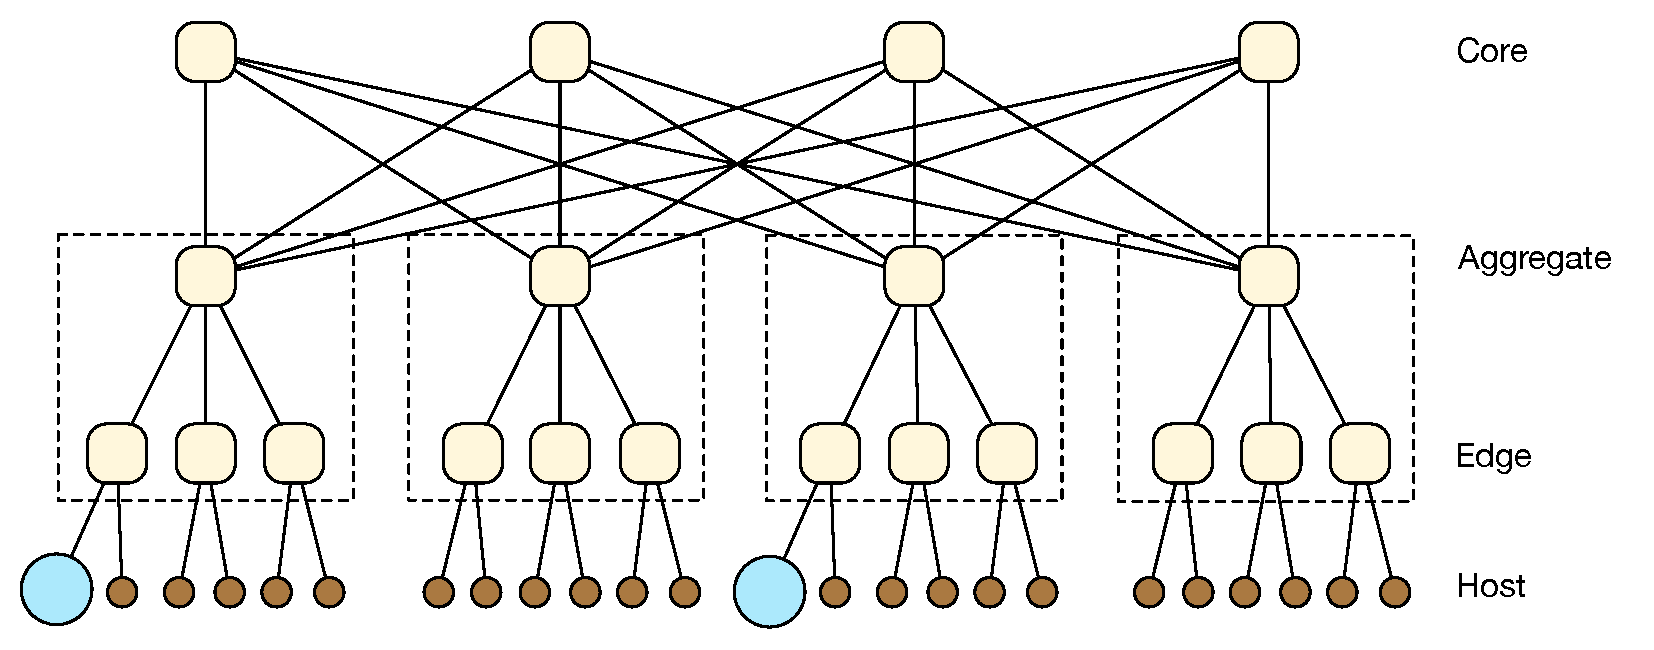
\includegraphics[width=0.45\textwidth]{figures/3-tier.eps}
 \caption{An instance of Canonical 3-Tiered topology with $k=4$. $k$ denotes the number of core switches. In this paper, the number of aggregate switches is also set to $k$, and each connects to $k-1$ edge switches. The total number of switches is $k^2 + k$. Each edge switch is directly connected to $\frac{k}{2}$ hosts. Therefore, there are $\frac{k^3 - k^2}{2}$ hosts in total.} 
 \label{topo_3tiered}
\end{figure}

\begin{figure}[!t]
\centering
 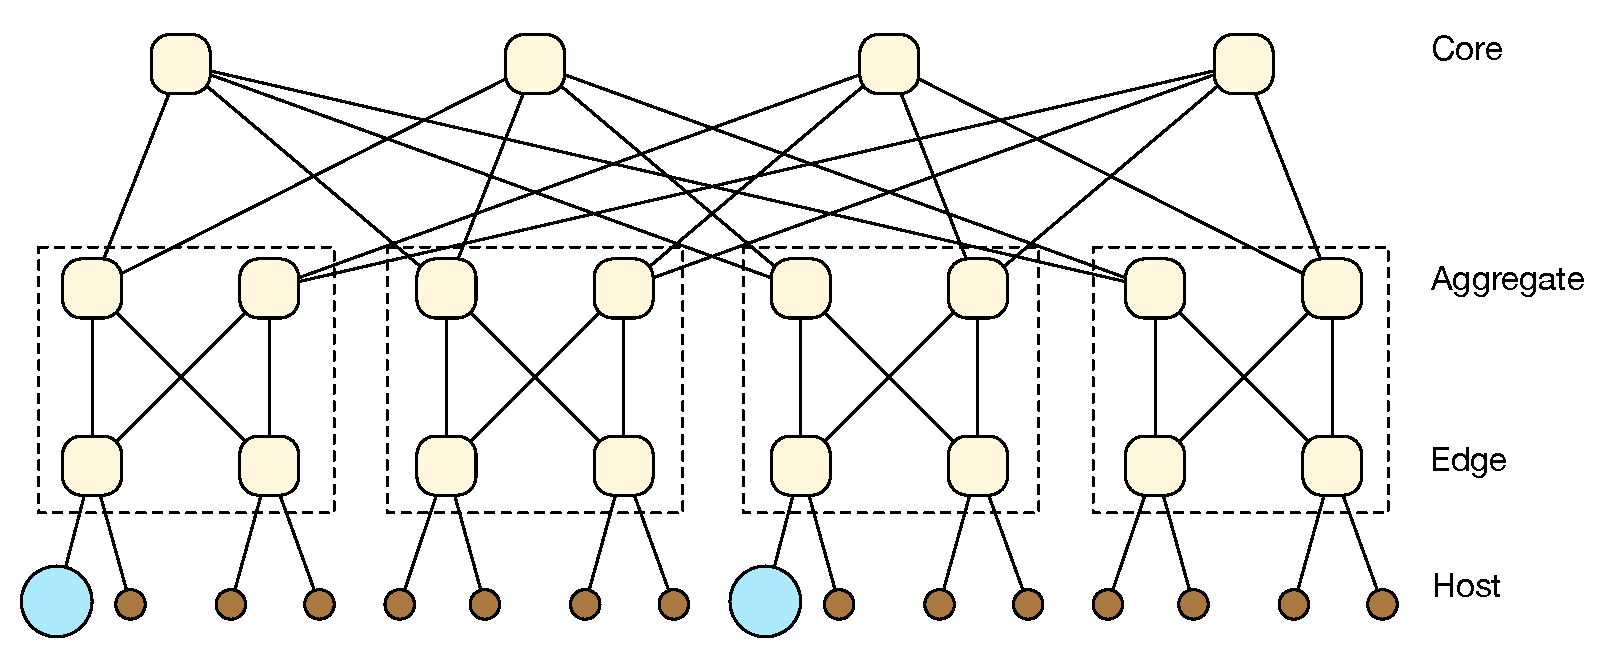
\includegraphics[width=0.45\textwidth]{figures/fattree.eps}
 \caption{An instance of Fat-tree topology with $k=4$. $k$ denotes the number of pods. The number of core, aggregate, edge switches are $\frac{k^2}{4}$, $\frac{k^2}{2}$, $\frac{k^2}{2}$, respectively. And the total number of switches is $\frac54 k^2$. Each edge switch is directly connected to $\frac{k}{2}$ hosts. Accordingly, there are $\frac{k^3}{4}$ hosts in total.}
\label{topo_fattree}
\end{figure}

In fact, there do exist hot spots within pods in real-world data center networks, where the switches have significantly high flow arrival rates. In our simulation, we pick the first pod as a hot spot and all switches there have significantly high flow arrival rate, i.e., $200$ flows per time slot. As for controllers, we set their individual capacity as $600$ flows per time slot. That is consistent with the capacity of a typical NOX controller \cite{tootoonchian2012controller}.

\textbf{Costs:} Given any network topology, we define the communication cost $W_{i,j}$ between switch $i$ and controller $j$ as the length (number of hops) of shortest path from $i$ to $j$. Then we set a common computation cost $\alpha$ for all switches, which equals to the average hop number between switches and controllers of its underlying topology. In Fat-tree topology, $\alpha = 4.13$; while in 3-Tiered topology, $\alpha = 4.81$.

\subsection{Evaluation of Greedy Algorithm}

Fig. \ref{trace}(a) presents how the summation of long-term average communication cost and computational cost changes with different $V$ in Fat-tree and 3-Tiered topologies. As $V$ varies from $0$ to $3.0 \times 10^7$, we can observe that the total cost goes down gradually. This is consistent with our previous theoretic analysis. The intuition behind such decline is as follows. Remind that $V$ controls the switches' willingness of uploading requests. For switches that are close to controllers (their communication cost is less than the average), large $V$ makes them unwilling to process requests locally unless the controllers get too heavy load. As $V$ increases, those switches will choose to upload requests to further reduce the costs since for those switches, communication costs are less than the computation cost. Another observation we make is that the total cost of 3-Tiered topology is more than Fat-tree's. The reason is that 3-Tiered has a higher computational cost ($\alpha = 4.81$ compared to $4.13$) and it cost more when switches process requests locally. In Fig. \ref{pp}(a), we also show the total cost of {\bf Greedy} in Fat-tree topology with other two request arrival processes. The curves of Poisson and Pareto exhibit qualitatively similar decline in total cost, although Pareto incurs slightly ($\sim 1.5\%$) larger queue backlog size than Poisson.

\begin{figure}[!t]
\centering
 \subfigure[Total cost vs. V] {
 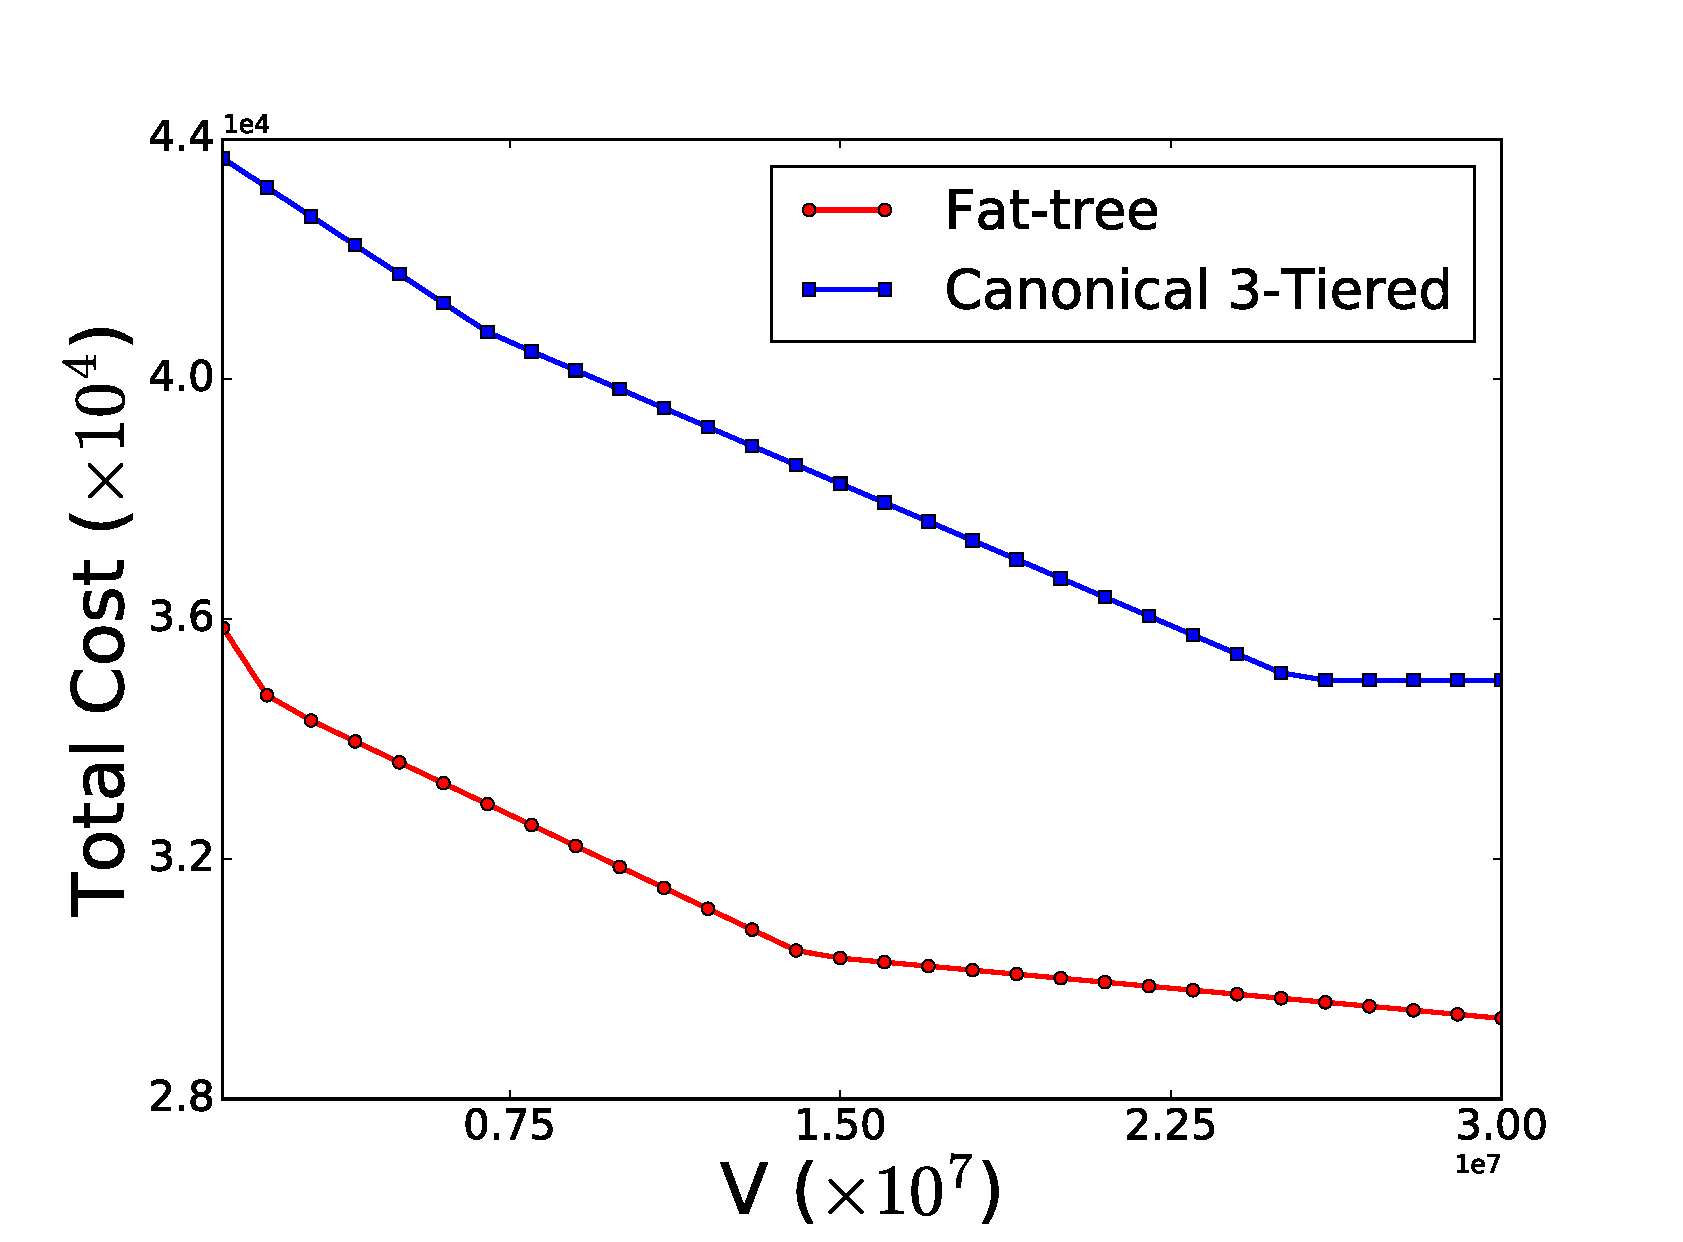
\includegraphics[width=0.465\columnwidth]{total_cost.eps}
 }
 \subfigure[Total queue backlog vs. V] {
 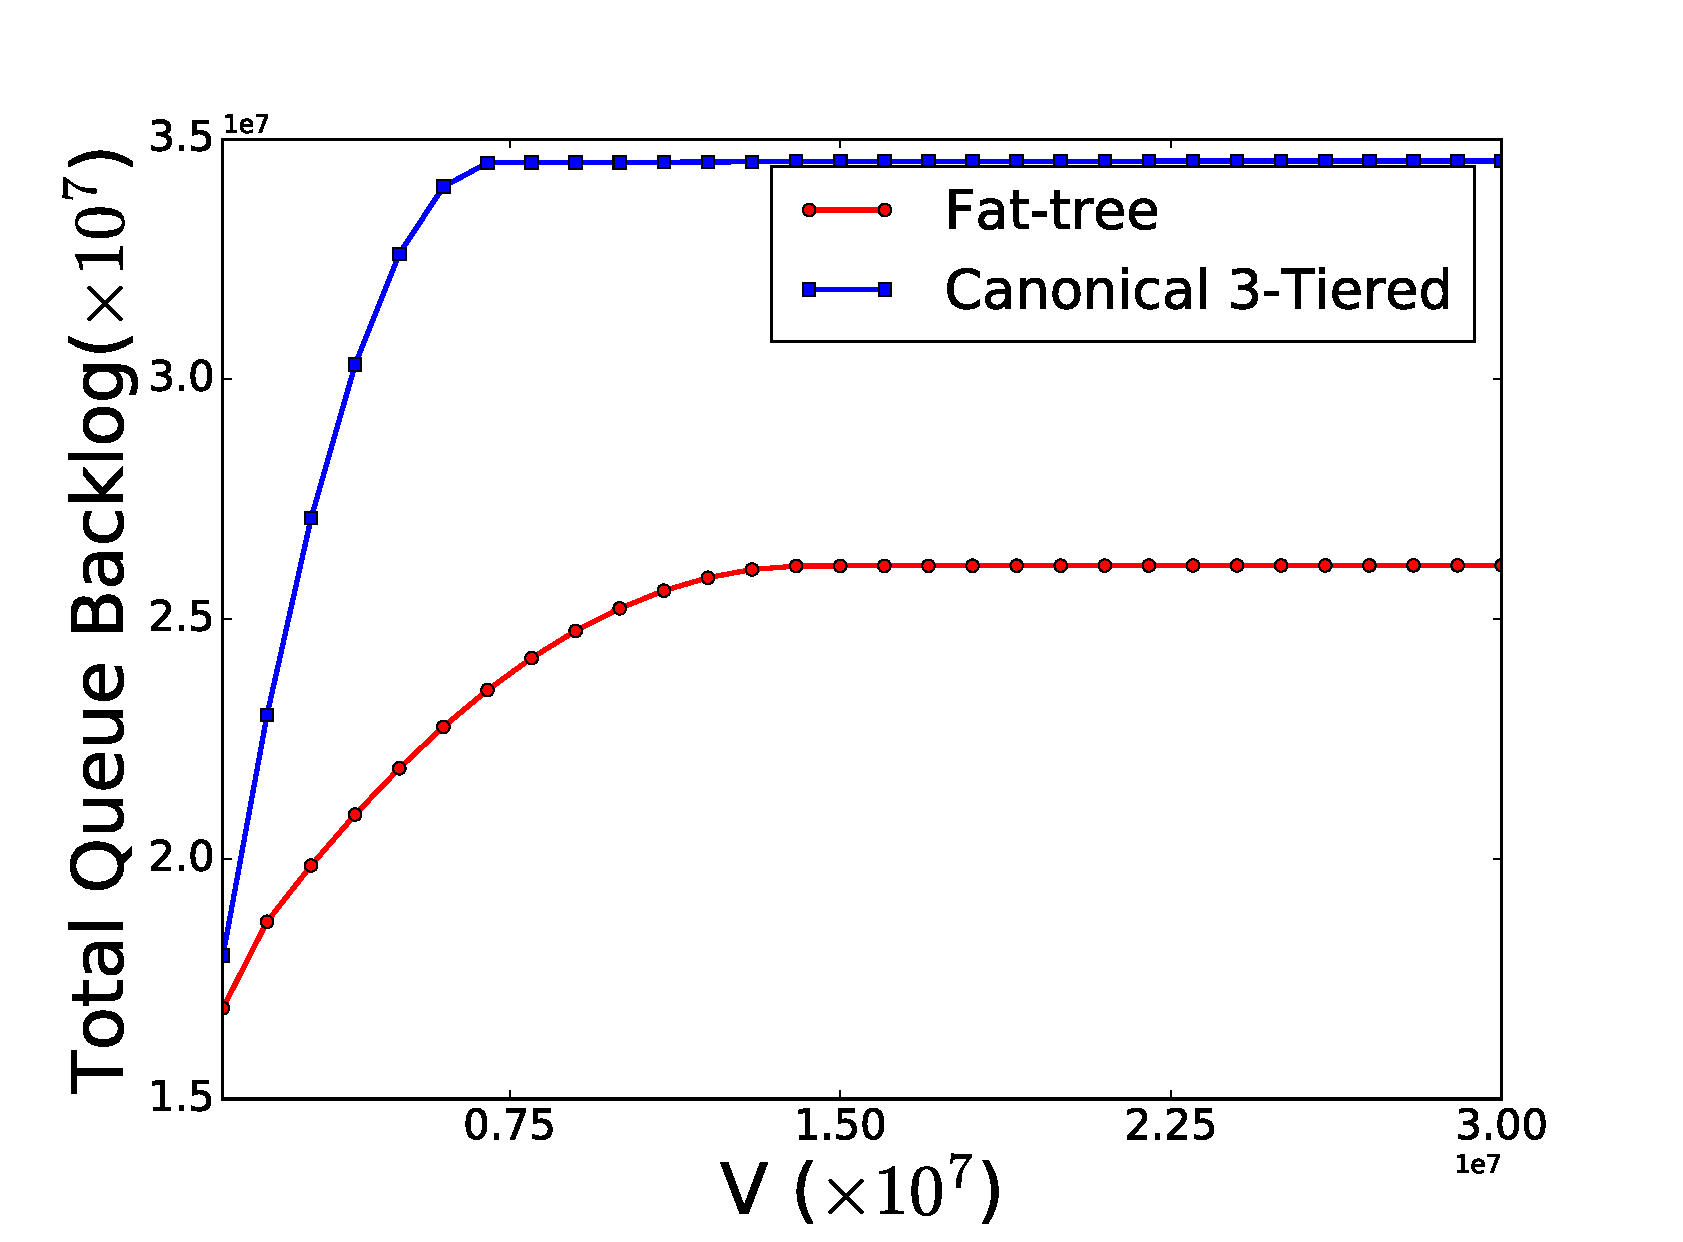
\includegraphics[width=0.465\columnwidth]{total_qlen.eps}
 }
 \caption{Performance of \textbf{Greedy} under Fat-tree topology and Canonical 3-Tiered topology in terms of (a) the sum of total communication cost and computational cost, and (b) total queue backlog.}
 \label{trace}
\end{figure}

\begin{figure}[!t]
	\centering
	\subfigure[Total cost vs. V] {
		\includegraphics[width=0.45\columnwidth]{total_cost_pp.eps}
	}	
	\subfigure[Total queue backlog vs. V] {
		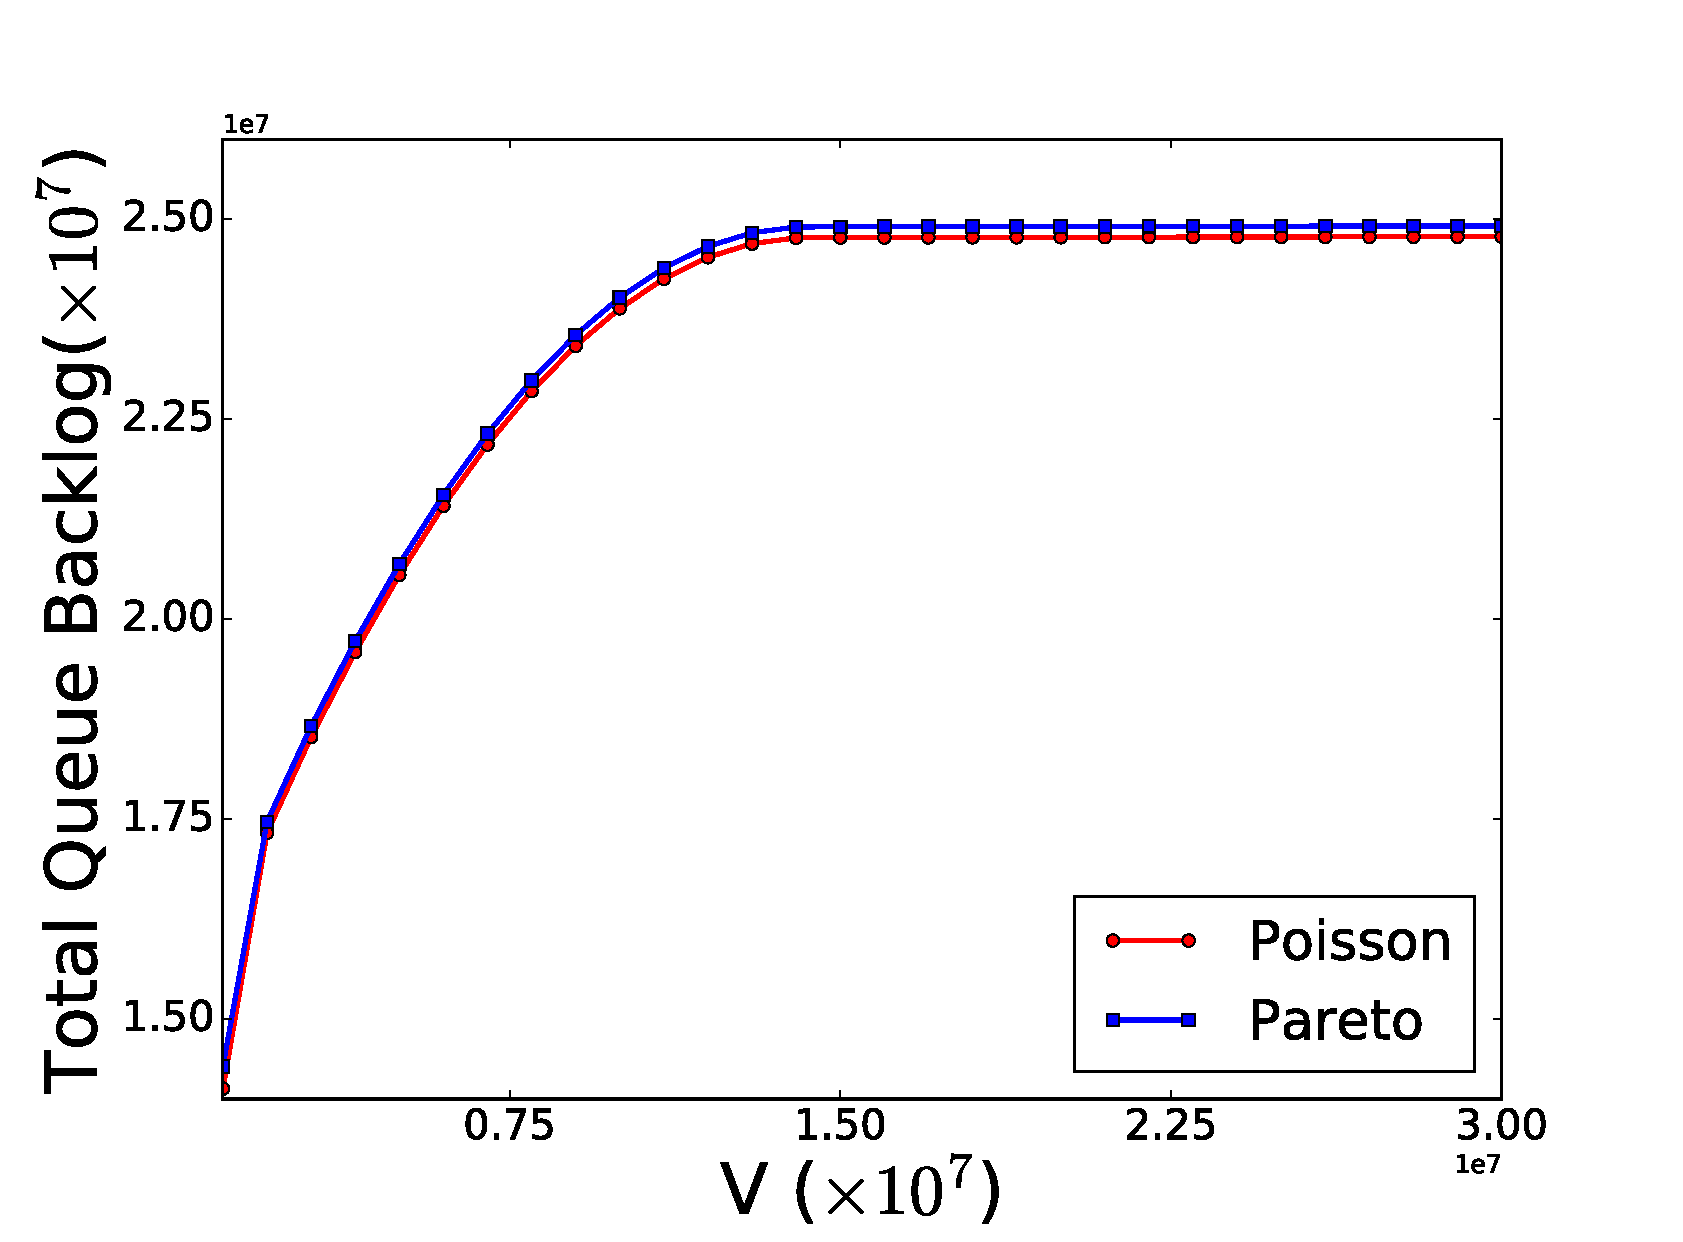
\includegraphics[width=0.45\columnwidth]{total_qlen_pp.eps}
	}
	
	\caption{Performance of \textbf{Greedy} under Fat-tree topology with request arrivals that follow Poisson and Pareto process in terms of (a) the sum of total communication cost and computational cost, and (b) total queue backlog.}
	\label{pp}
\end{figure}

Fig. \ref{trace}(b) shows the curve of total queue backlog size with different values of $V$. From the figure, we notice that total queue backlog size increases until $V$ reaches about $0.75 \times 10^7$ and $1.5 \times 10^7$ in Fat-tree and 3-Tiered topologies, respectively. This is also consistent with the $O(V)$ queue backlog size bound in (\ref{th1}). Recall our analysis in \emph{Total Cost}: larger $V$ invokes most switches to spend more time uploading requests to control plane. However, control plane's service capacity is fixed and requests will keep accumulating. Thus when $V$ becomes sufficiently large, control plane will eventually hold most of requests in the system. This explains the increasing queue backlog size in Fig. \ref{trace}(b). Fig. \ref{pp}(b) present the total queue backlog size in Fat-tree topology when we apply {\bf Greedy} with request arrivals that follow Poisson and Pareto processes. Note that we do not show that of 3-Tiered topology because curves there almost overlap with those in Fig. \ref{pp}(b).

\subsection{Comparison with Other Association Schemes}

In this subsection, we consider the extreme case by setting common computational cost $\alpha = 2.0 \times 10^{28}$ for all switches. This means the cost of local processing requests are prohibitively high and each time slot switches choose to upload requests to controllers. Thus our greedy algorithm degenerates into a dynamic switch-controller association algorithm. We compare its performance with three other schemes: \textbf{Static}, \textbf{Random} and \textbf{JSQ(Join-the-Shorest-Queue)}. In static scheme, each switch $i$ chooses the controller $j$ with minimum communication cost $W_{i,j}$ and then fixes this association for all time slots. In random scheme, the scheduler randomly picks up a controller for each switch at each time slot. In JSQ scheme, it randomly picks up one switch $i$ without replacement round by round until all switches have chosen the target controllers. At each round, the selected switch $i$ chooses the controller $j$ with the smallest queue backlog size at present, and appends all its requests to $j$'s queue. 

Fig. \ref{cost_trace} presents a comparison among \textbf{Static}, \textbf{Random}, \textbf{JSQ}, and \textbf{Greedy} in terms of communication cost under Canonical 3-Tiered topology and Fat-tree, respectively. First, the communication cost under \textbf{Static} is the minimum among all schemes, which is consistent with its goal of minimizing the overall communication cost. \textbf{Greedy} cuts down the communication cost with increasing $V$. Eventually, when $V$ is sufficiently large, communication cost stops decreasing and remains unchanged. Both \textbf{Random} and \textbf{JSQ} exhibit much higher communication costs, compared to \textbf{Greedy} and \textbf{Static}.

\begin{figure}[!t]
\centering
 \subfigure[Canonical 3-Tiered topology] {
 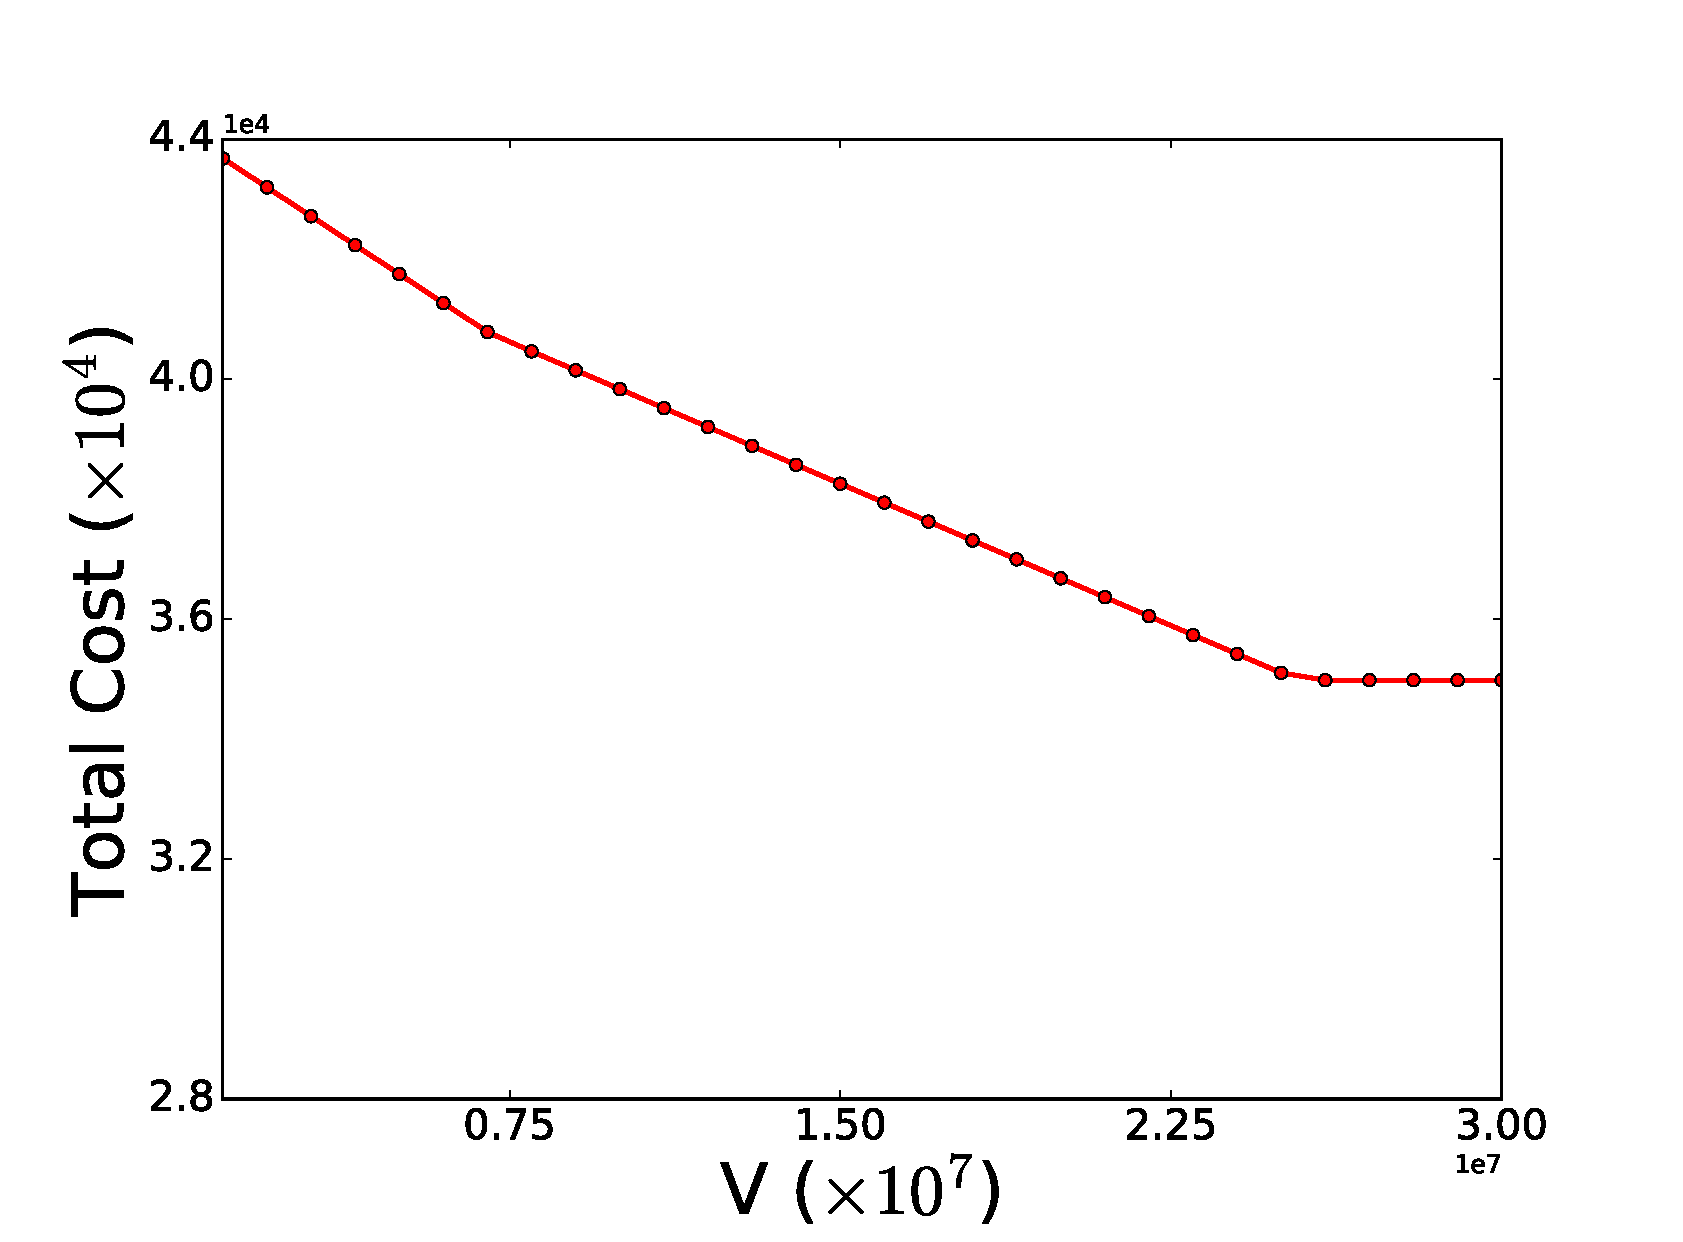
\includegraphics[width=0.465\columnwidth]{figures/60-trace-alpha-inf/total_cost_26.eps}
 }
 \subfigure[Fat-tree topology] {
 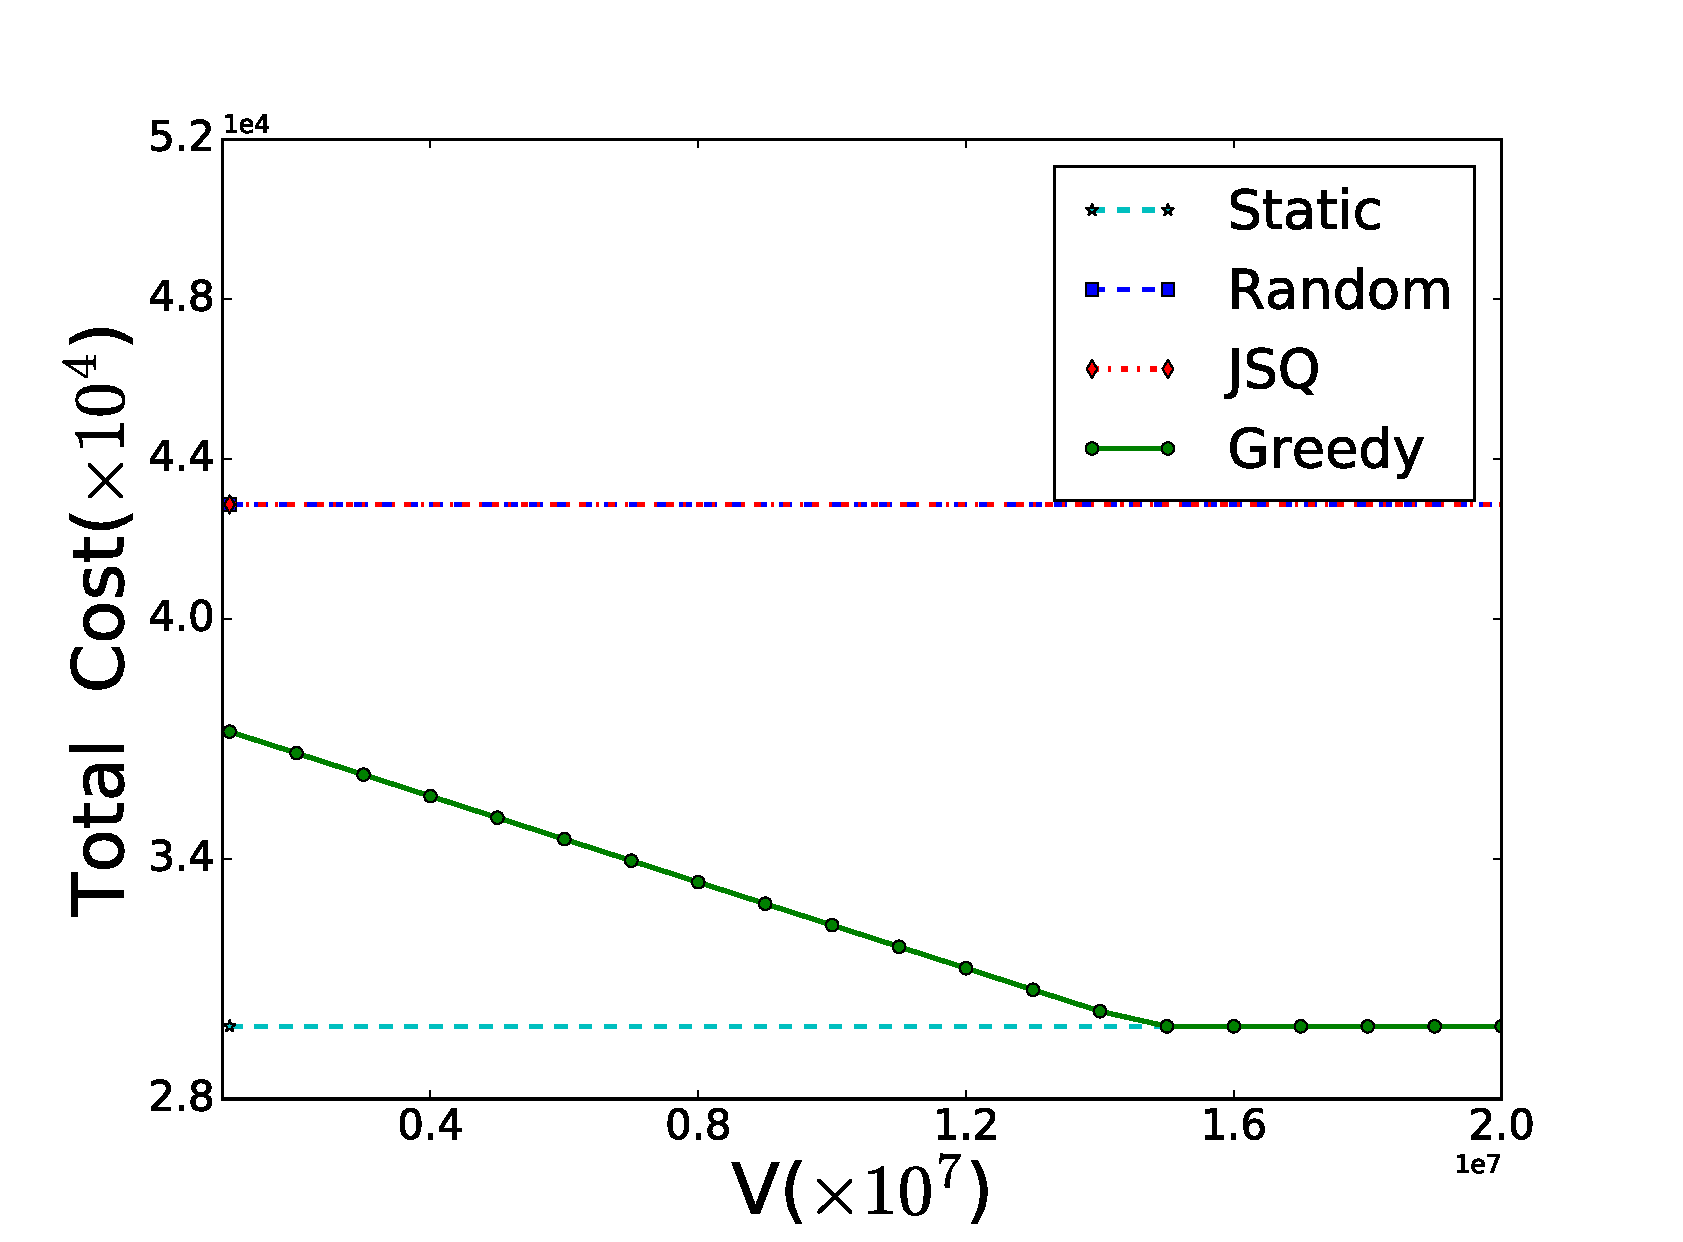
\includegraphics[width=0.465\columnwidth]{figures/10-trace-alpha-inf/total_cost_24.eps}
 }
 \caption{Communication cost comparison among four scheduling schemes under Canonical 3-Tiered topology and Fat-tree topology, respectively.}
 \label{cost_trace}
\end{figure}


\begin{figure}[!t]
\centering
 \subfigure[Canonical 3-Tiered topology] {
 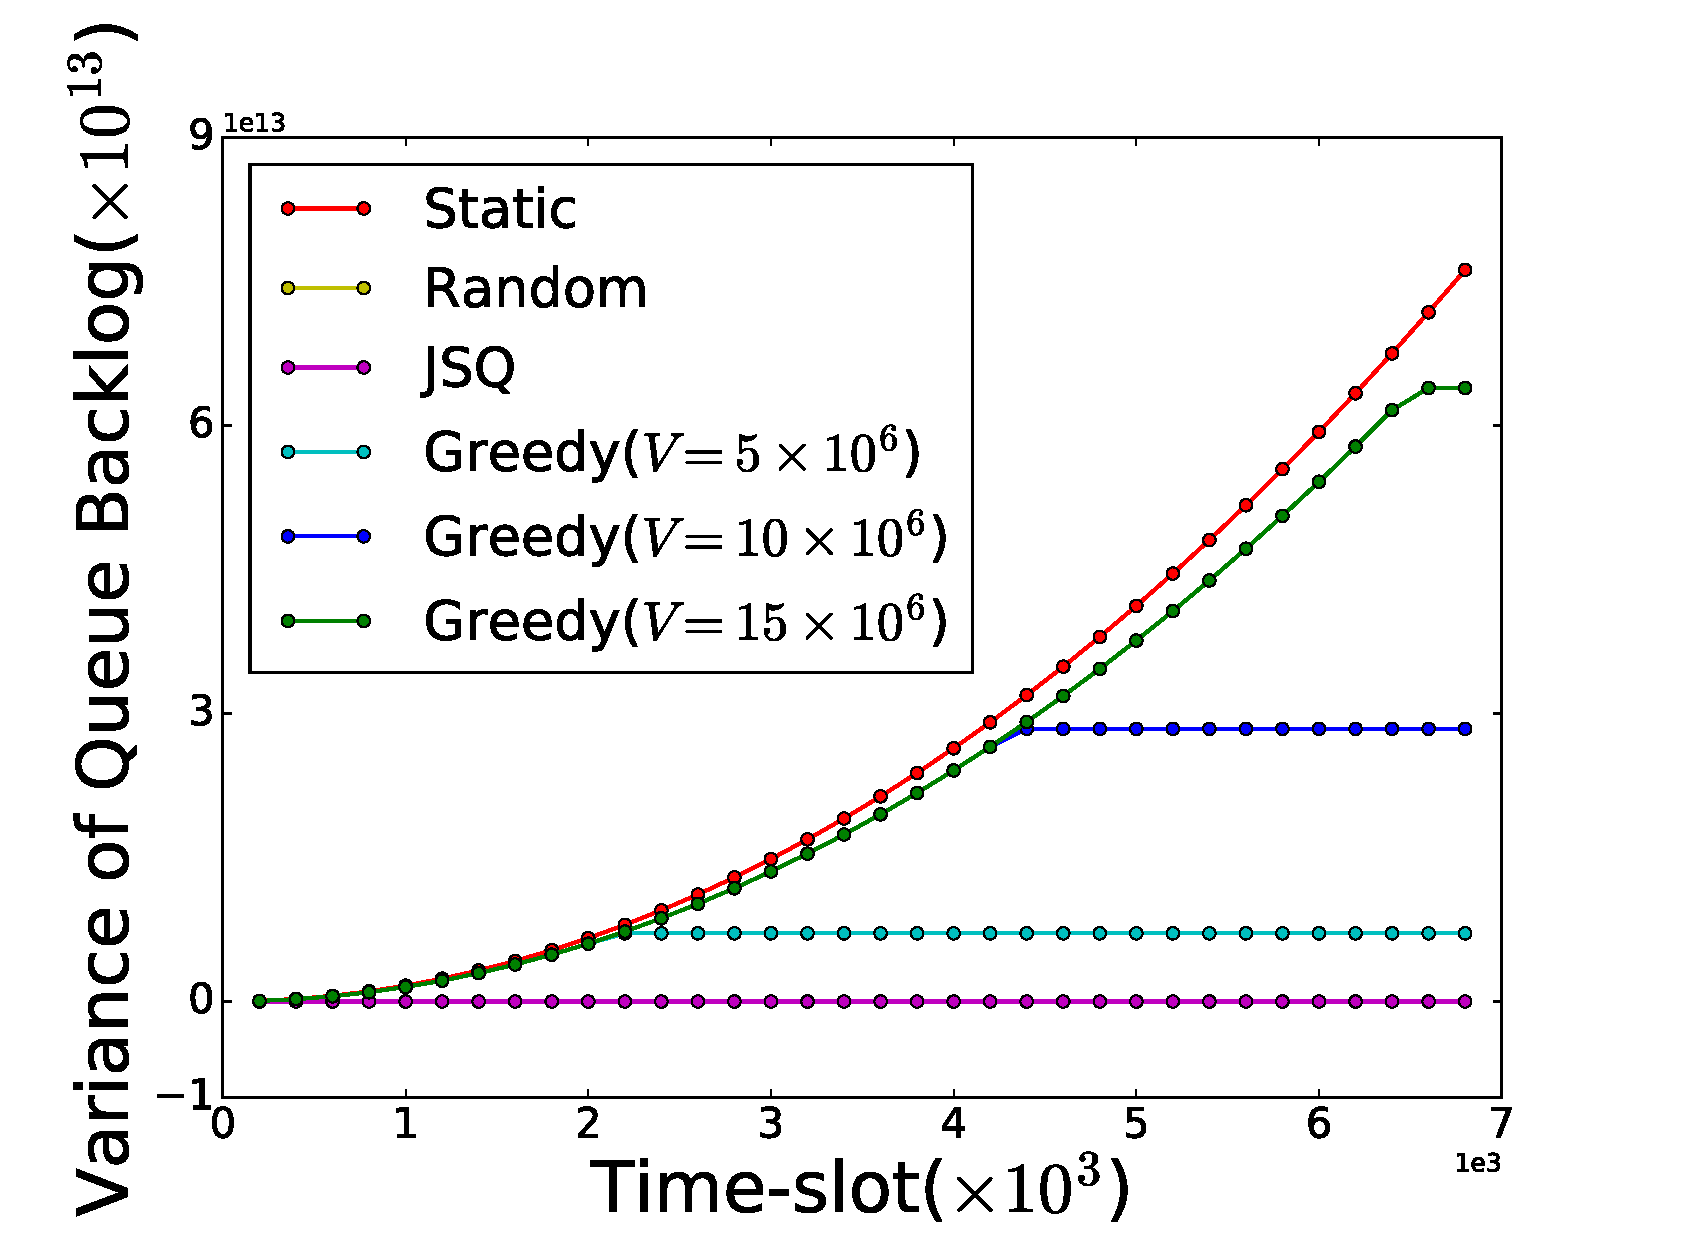
\includegraphics[width=0.465\columnwidth]{figures/60-trace-alpha-inf/var.eps}
 }
 \subfigure[Fat-tree topology] {
 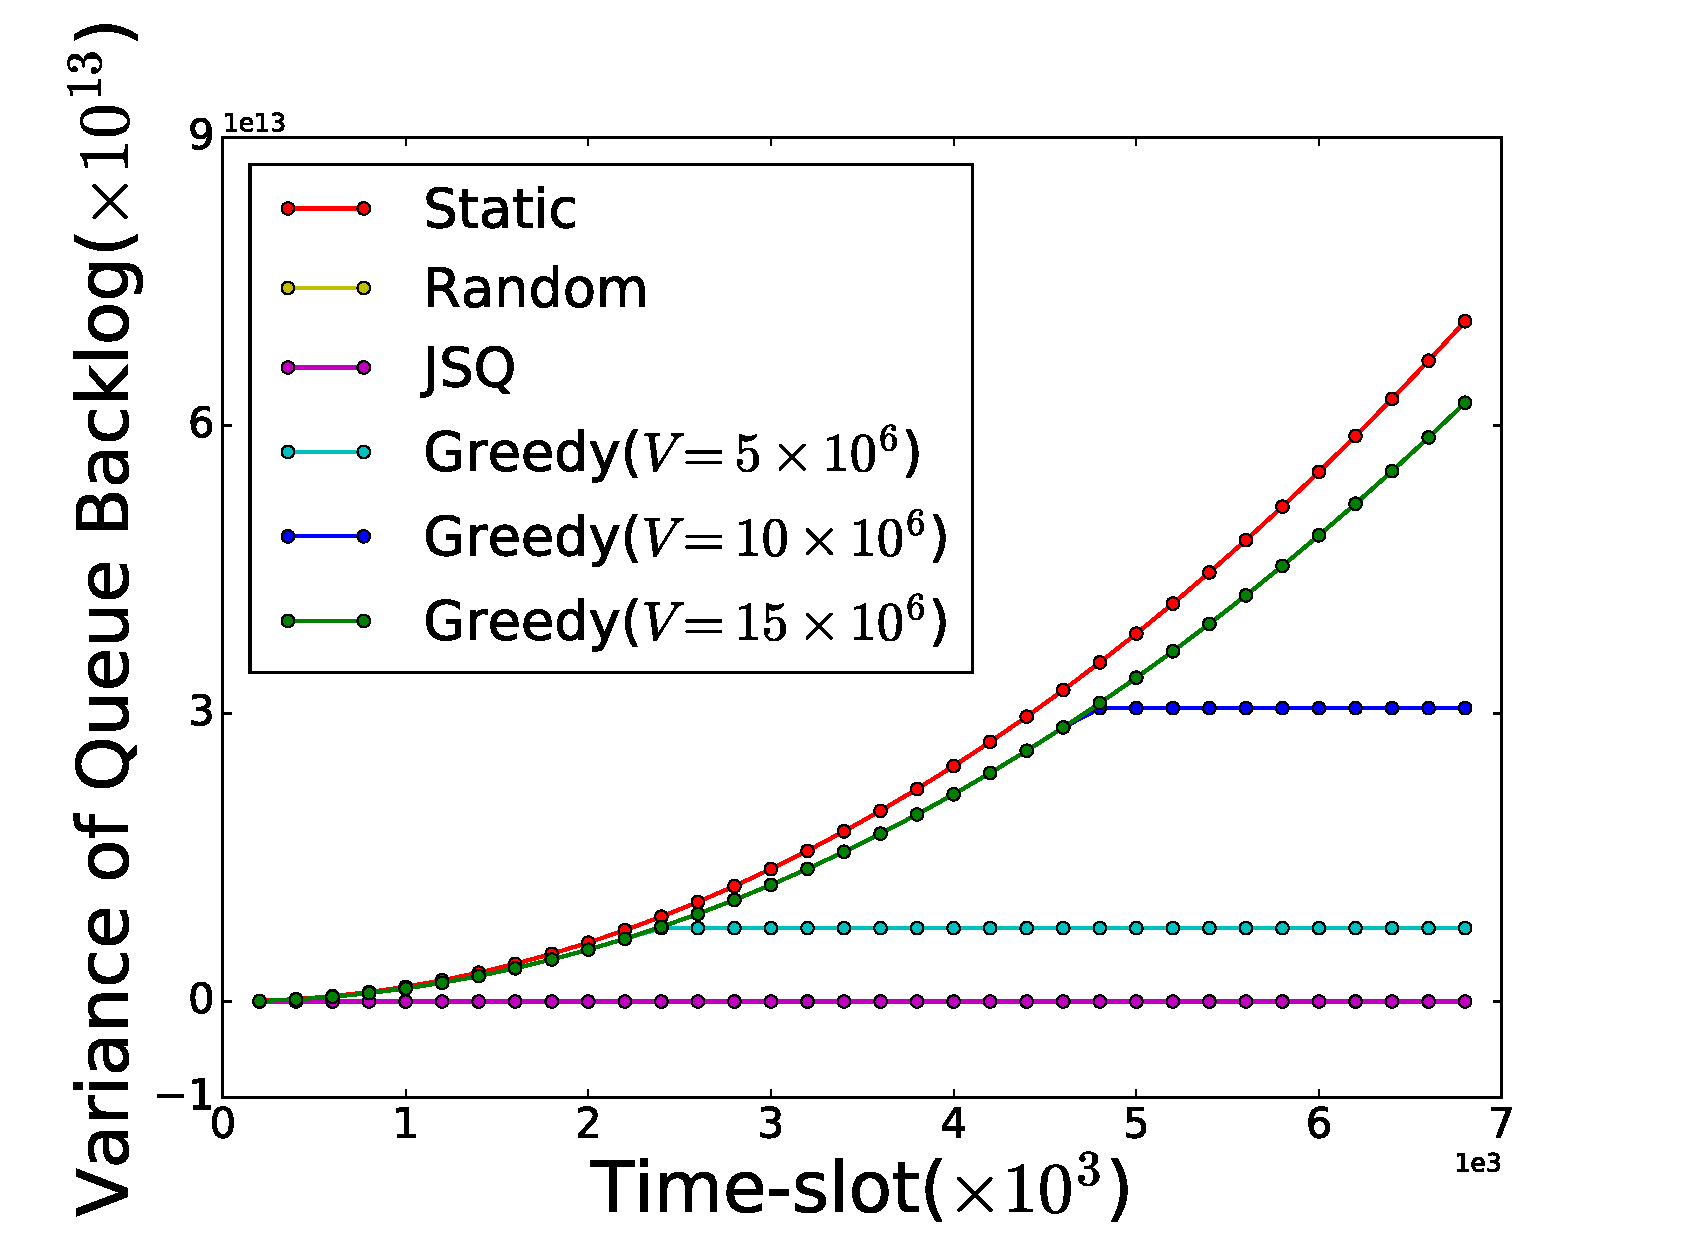
\includegraphics[width=0.465\columnwidth]{figures/10-trace-alpha-inf/var.eps}
 }
 \caption{Variance of queue backlog size comparison among four scheduling schemes under Canonical 3-Tiered topology and Fat-tree topology, respectively.}
 \label{var_trace}
\end{figure}

\begin{figure}[!t]
\centering
 \subfigure[Canonical 3-Tiered topology] {
 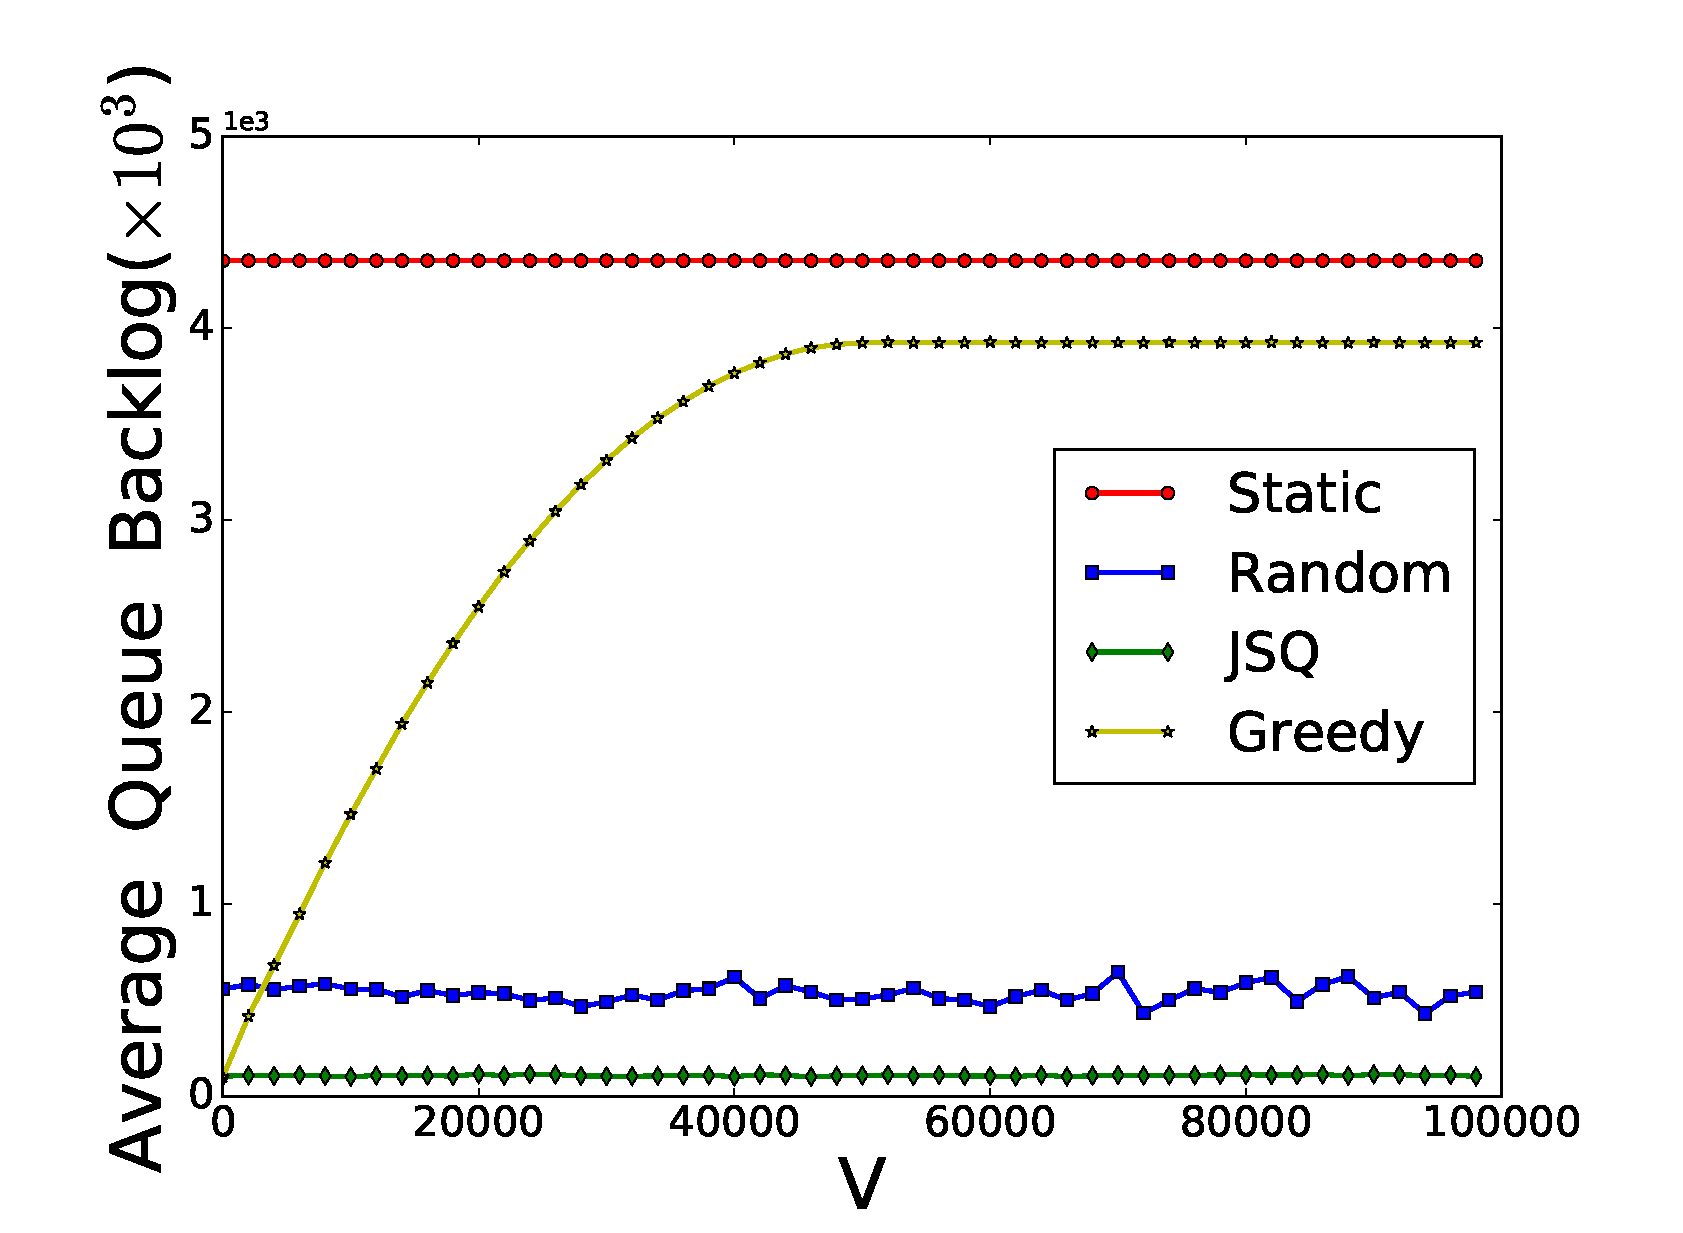
\includegraphics[width=0.465\columnwidth]{figures/60-trace-alpha-inf/qlen_3-tier.eps}
 }
 \subfigure[Fat-tree topology] {
 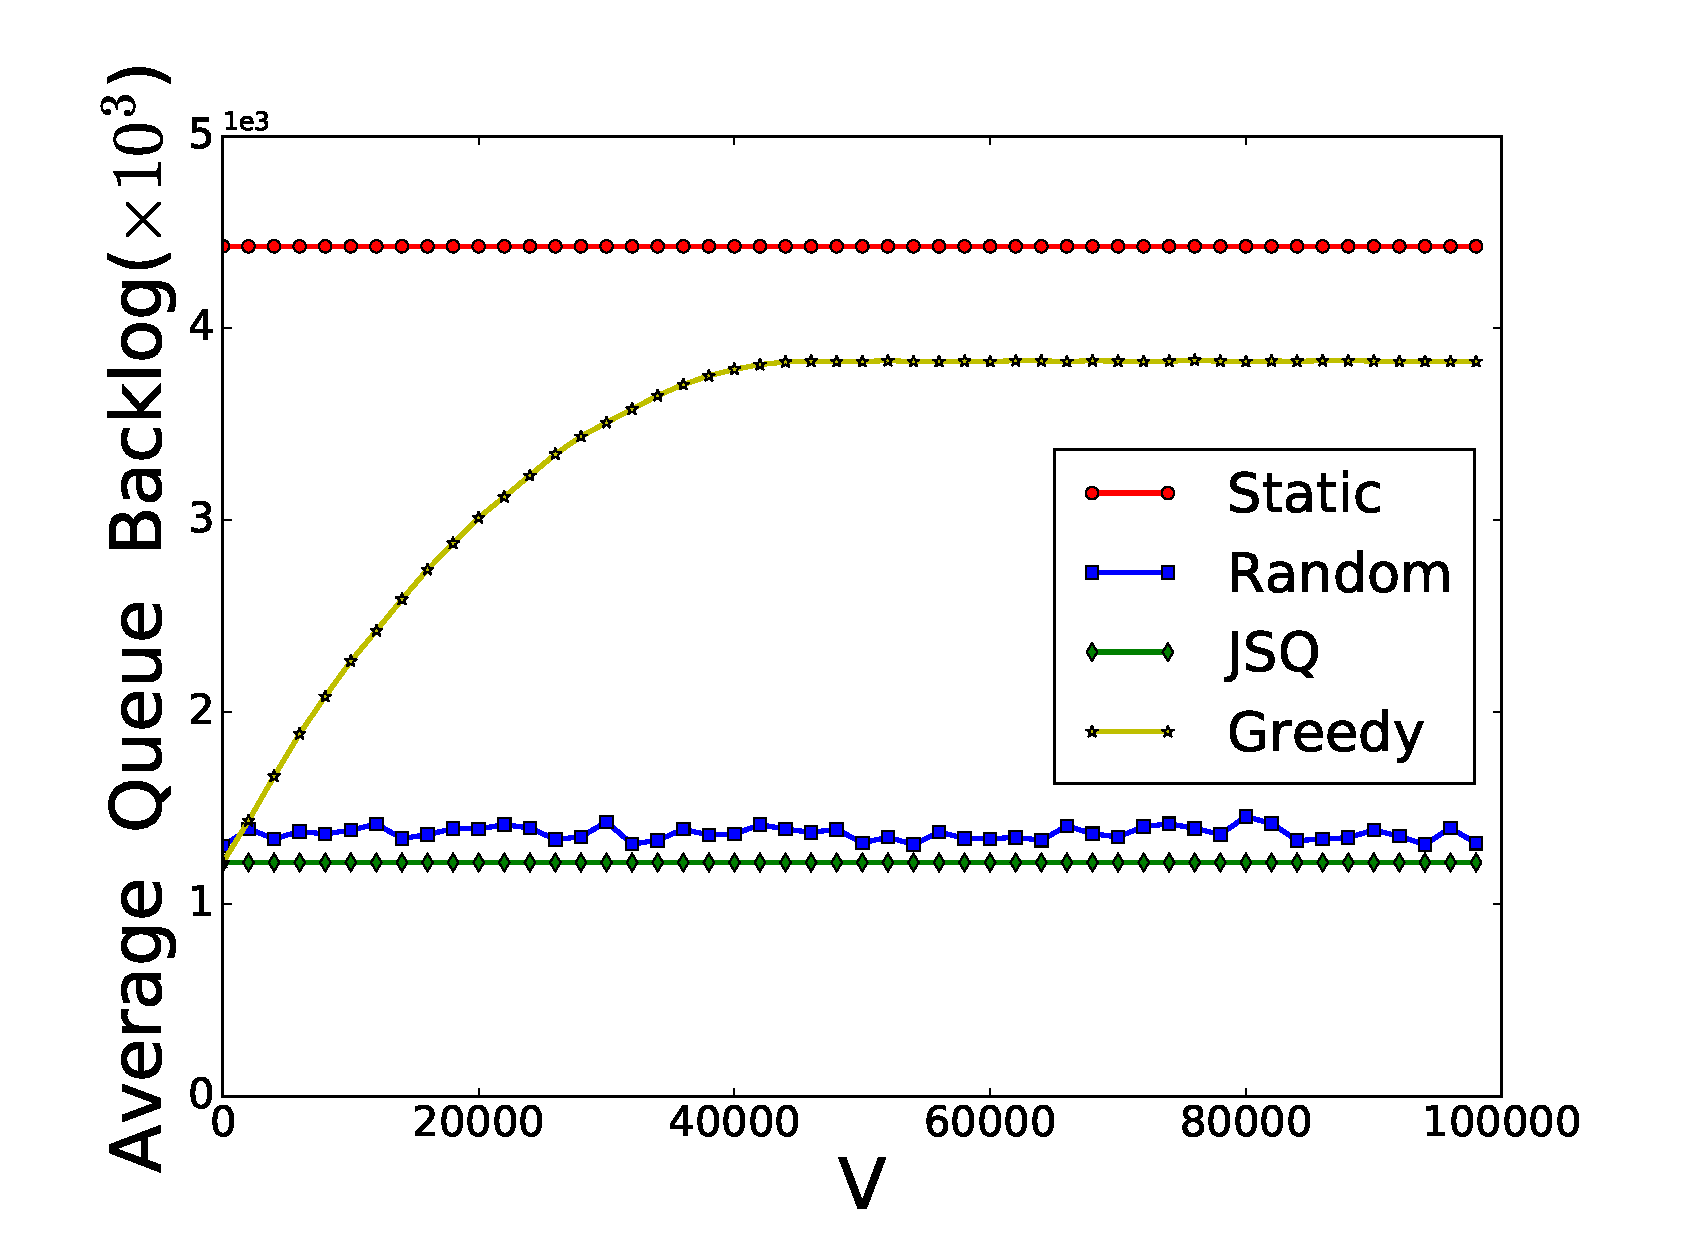
\includegraphics[width=0.465\columnwidth]{figures/10-trace-alpha-inf/qlen_fattree.eps}
 }
 \caption{Average queue backlog size comparison among four scheduling schemes under Canonical 3-Tiered topology and Fat-tree topology, respectively.}
 \label{qlen_trace}
\end{figure}

Fig. \ref{var_trace} presents a comparison among the four schemes in terms of the variance of queue backlog size under Canonical 3-Tiered topology and Fat-tree topology, respectively. In fact, smaller queue backlog size variance indicates better capability of load balancing. The variance of \textbf{Static} grows exponentially with time, showing that \textbf{Static} is incompetent in load balancing. The reason is that \textbf{Static} greedily associates switches with their nearest controllers, ignoring different controllers' loads. When it comes to \textbf{Random} and \textbf{JSQ}, the variance is almost $0$, which shows the two schemes' advantage in load balancing. While the variance of \textbf{Greedy} is in between the other three: it increases at the beginning and then remains stable after about thousands of time slots. Furthermore, \textbf{Greedy} exhibits higher variance of queue backlog size with larger $V$, i.e., the load of controllers is more imbalanced. 

Fig. \ref{qlen_trace} presents a comparison among the four schemes in terms of the average queue backlog size under Canonical 3-Tiered topology and Fat-tree topology, respectively. Actually, the observations in Fig. \ref{qlen_trace} are very consistent with that of Fig. \ref{var_trace}. Intuitively, the more balanced the load of controller is, the smaller of the average queue backlog size. In Fig. \ref{var_trace}, the variance of \textbf{Static} is high while that of \textbf{Random} and \textbf{JSQ} are almost $0$, so the average queue backlog size of \textbf{Static} is large while that of \textbf{Random} and \textbf{JSQ} is small in Fig. \ref{qlen_trace}. As for \textbf{Greedy}, the variance increases with $V$ in Fig. \ref{var_trace}, so the average queue backlog size of \textbf{Greedy}  rises as $V$ increases as shown in Fig. \ref{qlen_trace}.

\begin{figure}[!t]
\centering
 \subfigure[Poisson] {
 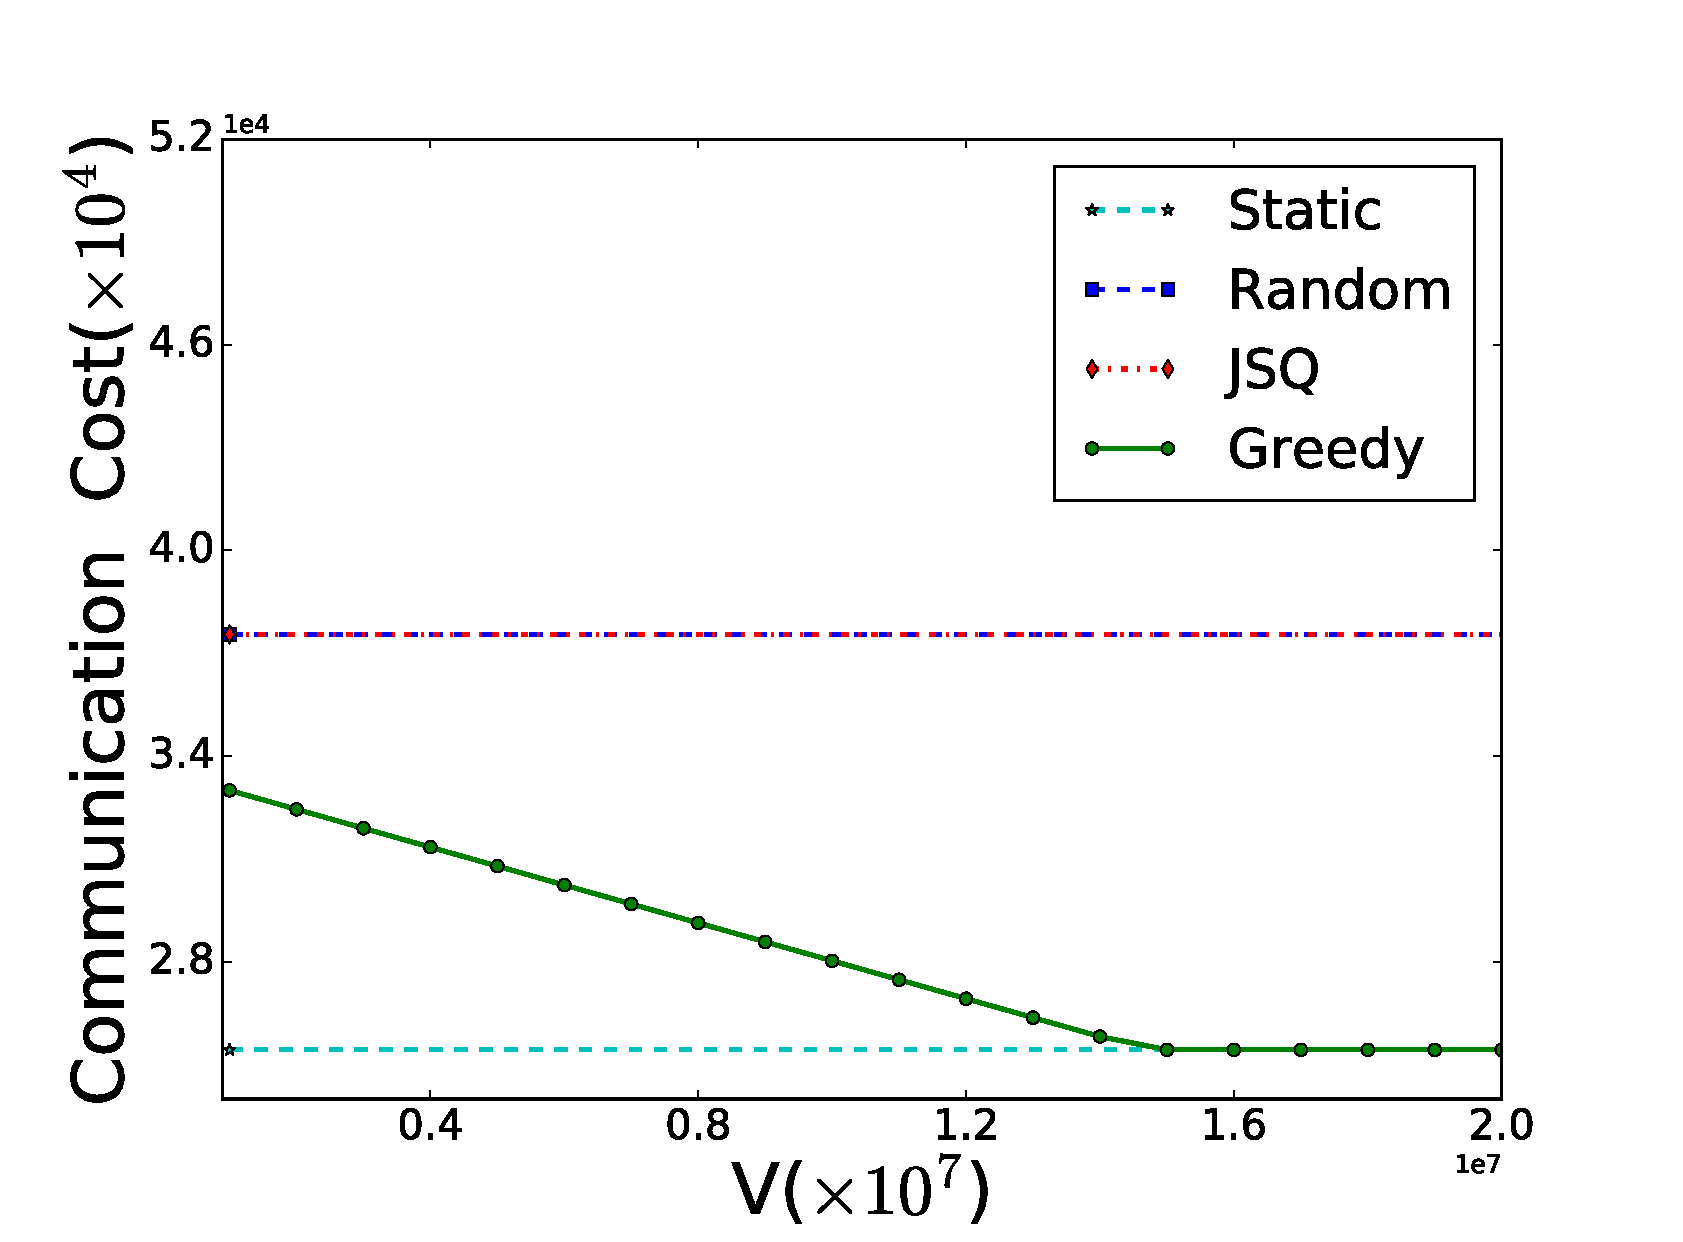
\includegraphics[width=0.465\columnwidth]{figures/10-exp-alpha-inf/cost_poisson.eps}
 }
 \subfigure[Pareto] {
 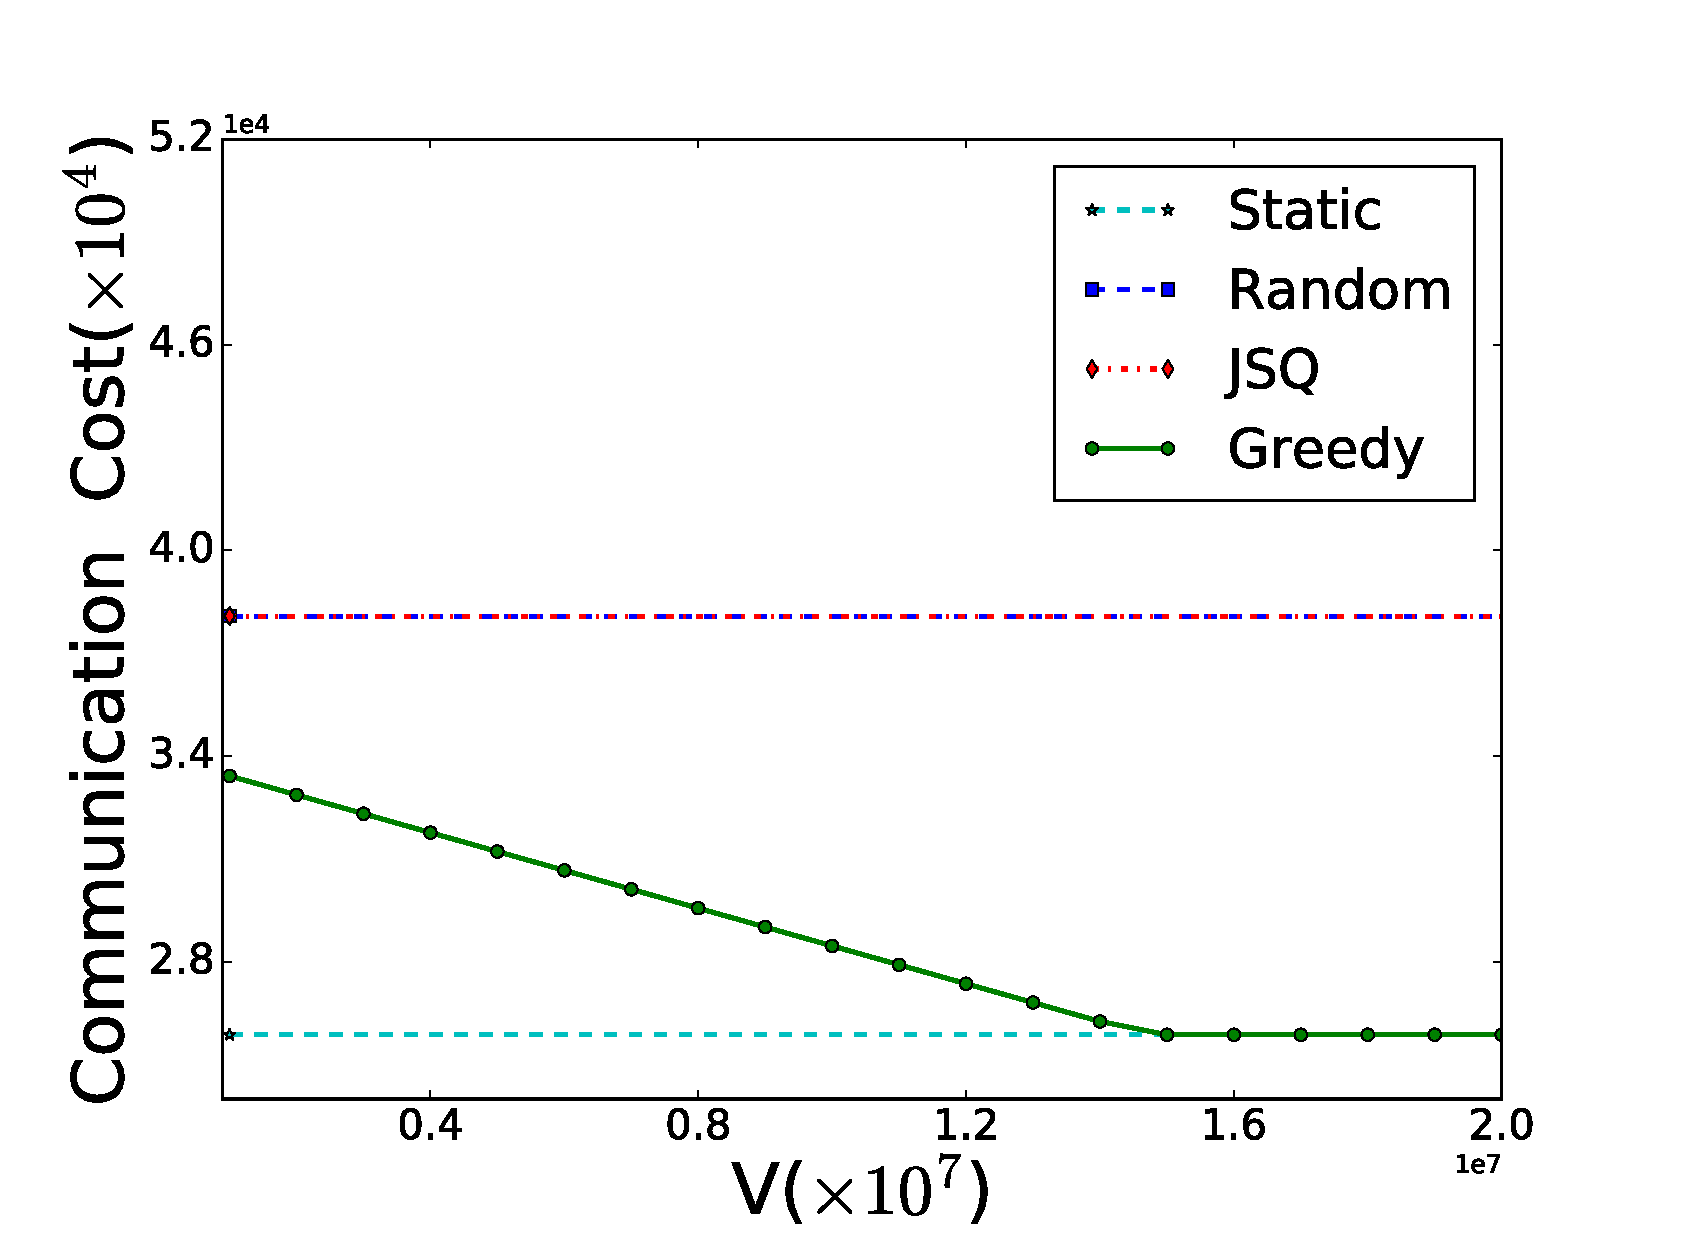
\includegraphics[width=0.465\columnwidth]{figures/10-pareto-alpha-inf/cost_pareto.eps}
 }
 \caption{Communication cost comparison among four scheduling schemes under Fat-tree topology, when the flow arrival follows Poisson and Pareto, respectively.}
 \label{cost}
\end{figure}

In addition to trace-driven simulation, we also conduct the comparison under other two assumptions of flow arrival processes, i.e., \emph{Poisson} and \emph{Pareto} processes. They two are widely adopted in traffic analysis. 
We only show the simulation results under Fat-tree topology, because the simulation results in 3-Tiered topology is qualitatively similar to that in Fat-tree topology.  Fig. \ref{cost} shows the communication cost comparison when the flow arrival process follows Poisson and Pareto, respectively. Fig. \ref{qlen} shows the average queue backlog size comparison when the flow arrival process follows Poisson and Pareto processes, respectively. We can see from these figures that the scheduling policies perform qualitatively consistent under different arrival processes.

In summary, among four schemes, \textbf{Static} is on the one end of performance spectrum: it minimizes communication cost while incurring extremely large queue backlogs; both \textbf{Random} and \textbf{JSQ} are on the other end of performance spectrum: they minimize the average queue backlog while incurring much large communication costs. In contrast, our \textbf{Greedy} scheme achieves a trade-off between minimization of communication costs and minimization of queue backlogs. Through a tunable parameter $V$, we can achieve different degrees of balance between cost minimization and latency (queue backlog) minimization. 

\begin{figure}[!t]
\centering
 \subfigure[Poisson] {
 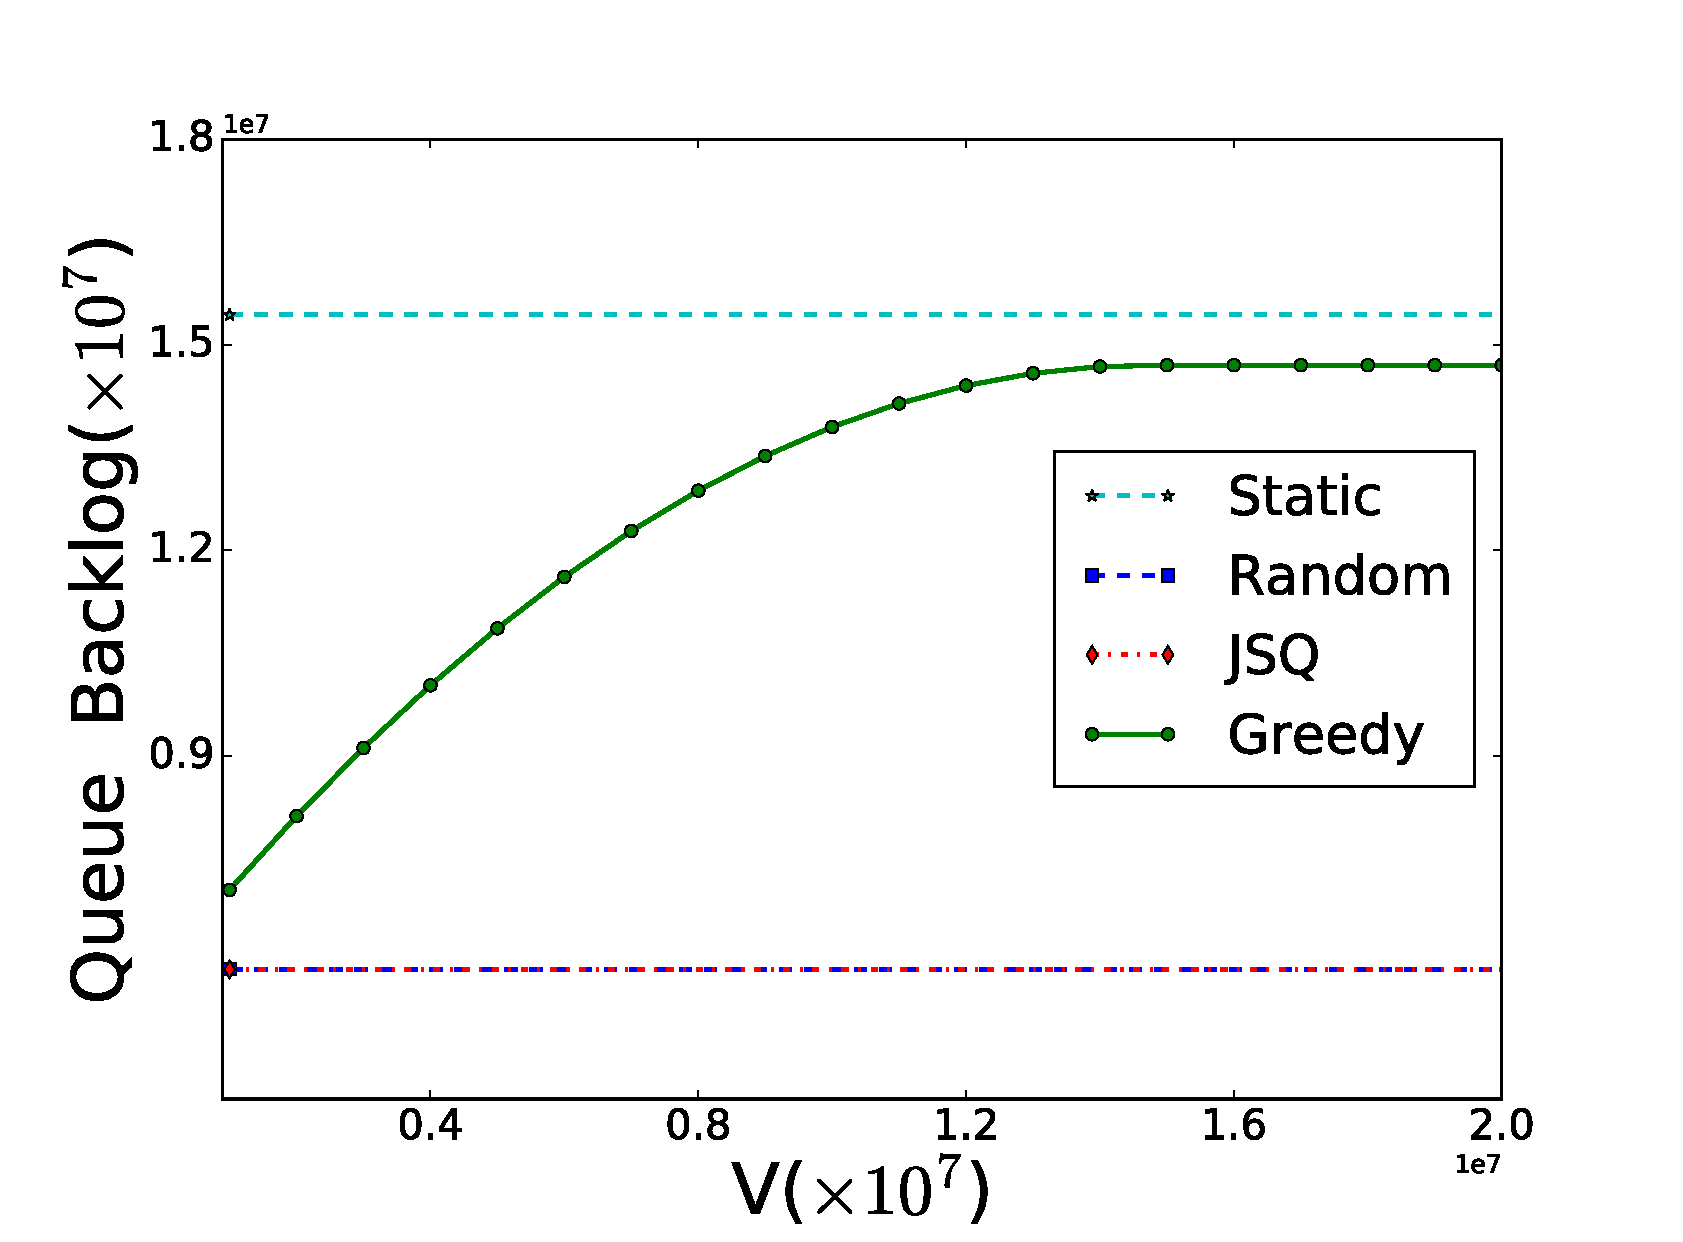
\includegraphics[width=0.465\columnwidth]{figures/10-exp-alpha-inf/qlen_poisson.eps}
 }
 \subfigure[Pareto] {
 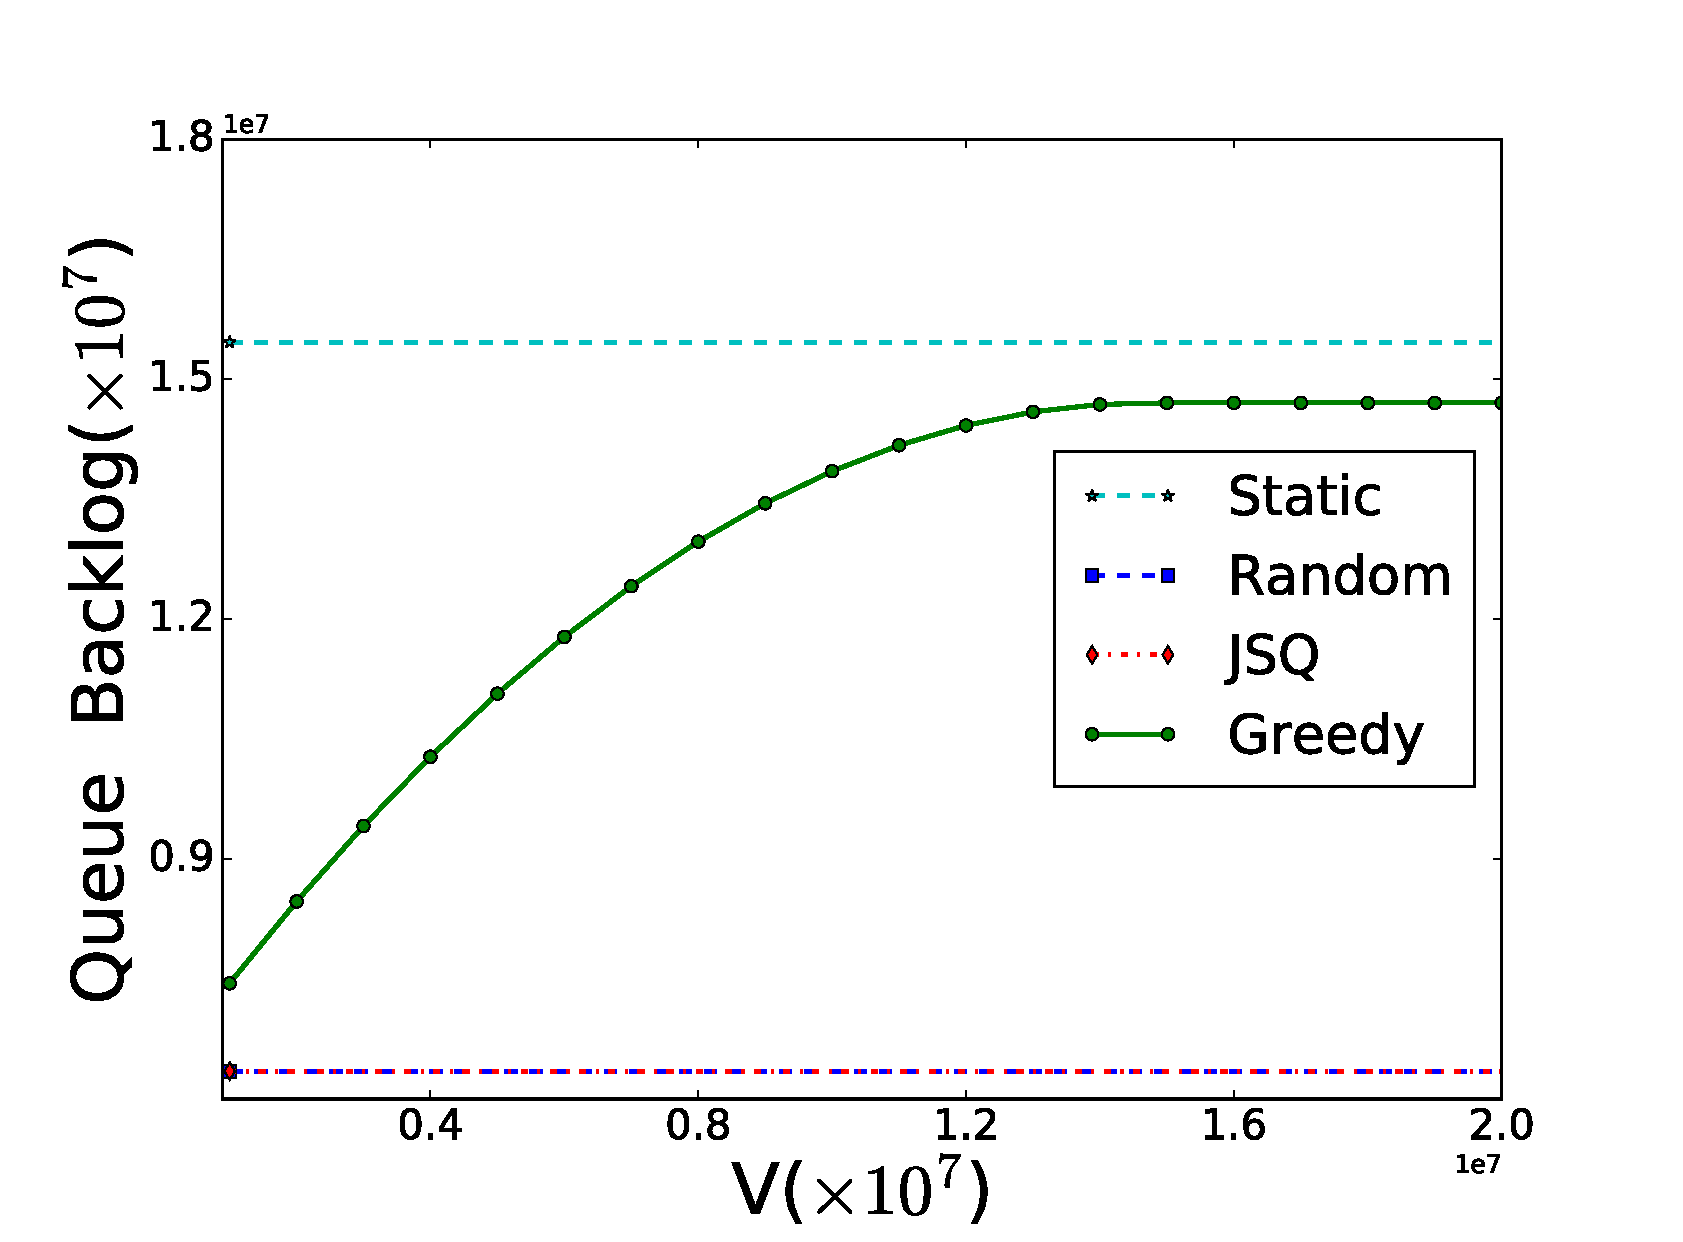
\includegraphics[width=0.465\columnwidth]{figures/10-pareto-alpha-inf/qlen_pareto.eps}
 }
 \caption{Average queue backlog size comparison among four scheduling schemes under Fat-tree topology, when the flow arrival follows Poisson and Pareto, respectively.}
 \label{qlen}
\end{figure}


\section{Conclusion}

In this paper, we studied the joint optimization problem of dynamic switch-controller association and dynamic control devolution for SDN networks. We formulated the problem as a stochastic network optimization problem, aiming at minimizing the long-term average summation of total communication cost and computational cost while maintaining low time-average queue backlogs. We proposed an efficient online greedy algorithm, which yields a long-term average sum of communication cost and computational cost within $O(1 \slash V)$ of optimality, with a trade-off in an $O(V)$ queue backlog size for any positive control parameter $V$. Extensive simulation results show the effectiveness and optimality of our online algorithm, and the ability to maintain a tunable trade-off compared to other dynamic association schemes. 


\appendices
\section{Problem Transformation by Opportunistically Minimizing an Expectation}

By minimizing the upper bound of the drift-plus-penalty expression (\ref{cond-v-drift}), the time average of communication cost can be minimized while stabilizing the network of request queues. 
We denote the objective function of (\ref{opt-pr}) at time slot $t$ by $J_t(\mathbf{X})$ and its optimal solution $\mathbf{X}^* \in \mathcal{A}$.

Therefore, for any other scheduling decision $\mathbf{X} \in \mathcal{A}$ made during time slot $t$, we have
\begin{equation}
	\begin{array}{c}
		J_t(\mathbf{X}) \ge J_t(\mathbf{X}^*)
	\end{array}
\end{equation}
Taking the conditional expectation on both sides conditional on $\mathbf{Q}^c(t)$, we have
\begin{equation}
	\begin{array}{c}
		E\left[J_t(\mathbf{X})\,|\,\mathbf{Q}^c(t)\right] \ge E\left[J_t(\mathbf{X}^*)\,|\,\mathbf{Q}^c(t)\right]
	\end{array}
\end{equation}
for any $\mathbf{X} \in \mathcal{A}$. In such way, instead of directly solving the long-term stochastic optimization problem (\ref{ori-opt-pr}), we can opportunistically choose a feasible association to solve problem (\ref{opt-pr}) during each time slot. 

\section{Proof of Theorem 1}
Given $L(\mathbf{Q}(t))$ defined in (\ref{lyqueue}), we have 
\begin{equation}\label{lyap-diff}
	\begin{array}{cl}
		& L(\mathbf{Q}(t+1)) - L(\mathbf{Q}(t)) \\
		= & \displaystyle \frac{1}{2} \left( \sum_{j \in \mathcal{C}} \left[ \left(Q^c_j(t+1)\right)^2 - \left(Q^c_j(t)\right)^2 \right] + \sum_{i \in \mathcal{S}} \left[ \left(Q^s_i(t+1)\right)^2 - \right. \right. \\
		& \displaystyle \left. \left. \left(Q^s_i(t)\right)^2 \right] \right) \\
		\le & \displaystyle \frac{1}{2} \sum_{j \in \mathcal{C}} \left\{ \left( Q^c_j(t) - B_j(t) + \sum_{i \in \mathcal{S}} \mathbf{X}_{i,j} \cdot {A}_{i}(t) \right)^2 - \left(Q^c_j(t)\right)^2 \right\} + \\
		& \displaystyle \frac{1}{2} \sum_{i \in \mathcal{S}} \left\{ \left( Q^s_i(t) - U_i(t) + \mathbf{Y}_i \cdot {A}_{i}(t) \right)^2 - \left(Q^s_i(t)\right)^2 \right\} \\
		= & \displaystyle \frac{1}{2} \sum_{j \in \mathcal{C}} \left\{ 2Q^c_j(t) \cdot \left( \sum_{i \in \mathcal{S}} \mathbf{X}_{i,j}\cdot {A}_{i}(t) - B_j(t) \right) + \right. \\
		& \displaystyle \left. \left( \sum_{i \in \mathcal{S}} \mathbf{X}_{i,j} \cdot {A}_{i}(t) - B_j(t) \right)^2 \right\} + 
		\frac{1}{2} \sum_{i \in \mathcal{S}} \displaystyle \left\{ \left( \mathbf{Y}_i \cdot {A}_{i}(t) - U_i(t) \right)^2 \right. \\
		& \displaystyle \left. + 2Q^s_i(t) \cdot \left( \mathbf{Y}_i \cdot {A}_{i}(t) - U_i(t) \right) \right\}
		\\
		\le & \displaystyle \sum_{j \in \mathcal{C}} \left\{ Q^c_j(t) \cdot \left( \sum_{i \in \mathcal{S}} \mathbf{X}_{i,j} \cdot {A}_{i}(t) - B_j(t) \right) + \right. \\
		& \displaystyle \left. \frac{ (\sum_{i \in \mathcal{S}} \mathbf{X}_{i,j}\cdot {A}_{i}(t))^2 + (B_j(t))^2}{2} \right\} + \\
		& \displaystyle \sum_{i \in \mathcal{S}} \left\{ Q^s_i(t) \cdot \left( \mathbf{Y}_{i} \cdot {A}_{i}(t) - U_i(t) \right) +
		\frac{ (Y_i \cdot {A}_{i}(t))^2 + (U_i(t))^2}{2} \right\} \\
	\end{array}	
\end{equation}


Then with the definition of $\Delta(\mathbf{Q}(t))$ in (\ref{cond-drift}), we have
\begin{equation}\label{lyap-delta1}
	\begin{array}{cl}
		& \Delta(\mathbf{Q}(t)) \\
		= & E\left\{ L\left(\mathbf{Q}(t+1)\right) - L\left( \mathbf{Q}(t) \right)\,|\,\mathbf{Q}(t) \right\} \\
		\le & \displaystyle E\left\{ \sum_{j \in \mathcal{C}} Q^c_j(t) \cdot \left( 
		\sum_{i \in \mathcal{S}} \mathbf{X}_{i,j}(t) A_i(t) - B_j(t)
		\right) \,|\, \mathbf{Q}(t) \right\} + \\
		  & \displaystyle E\left\{ \sum_{i \in \mathcal{S}} Q^s_i(t) \cdot \left( 
		\mathbf{Y}_{i}(t) A_i(t) - U_i(t)
		\right) \,|\, \mathbf{Q}(t) \right\} + \\
		& \displaystyle \frac{1}{2} E \left\{ \sum_{j \in \mathcal{C}} \left[ \left( \sum_{i \in \mathcal{S}} \mathbf{X}_{i,j} A_i(t) \right)^2  + \left( B_j(t) \right)^2 \right] \,|\,\mathbf{Q}(t) \right\} + \\
		& \displaystyle \frac{1}{2} E \left\{  \sum_{i \in \mathcal{S}} \left[ \left( \mathbf{Y}_{i} A_i(t) \right)^2  + \left( U_i(t) \right)^2 \right] \,|\,\mathbf{Q}(t) \right\} \\
		= & \displaystyle \sum_{j \in \mathcal{C}} Q^c_j(t) \cdot E \left\{ \left( 
		\sum_{i \in \mathcal{S}} \mathbf{X}_{i,j}(t) A_i(t) - B_j(t)
		\right) \,|\, \mathbf{Q}(t) \right\} + \\
		  & \displaystyle \sum_{i \in \mathcal{S}} Q^s_i(t) \cdot E \left\{ \left( 
		\mathbf{Y}_{i}(t) A_i(t) - U_i(t)
		\right) \,|\, \mathbf{Q}(t) \right\} + \\
		& \displaystyle \frac{1}{2} \sum_{j \in \mathcal{C}} \left[ \left( \sum_{i \in \mathcal{S}} \mathbf{X}_{i,j} A_i(t) \right)^2  + \left( B_j(t) \right)^2 \right] + \\
		& \displaystyle \frac{1}{2} \sum_{i \in \mathcal{S}} \left[ \left( \mathbf{Y}_{i} A_i(t) \right)^2  + \left( U_i(t) \right)^2 \right] \\
	\end{array}
\end{equation}
The last equality in (\ref{lyap-delta1}) holds because of conditional expectation on $\mathbf{Q}(t)$, then both $Q_i^s(t)$ and $Q_j^c(t)$ can be regarded as a constant. Besides, the queueing process $\{\mathbf{Q}(t)\}$ is independent of the arrival process $\{\mathbf{A}(t)\}$ and service process $\{\mathbf{B}(t)\}$, $\{\mathbf{U}(t)\}$. Hence, the last two terms have nothing to do with $\mathbf{Q}(t)$. Now consider the last two terms in (\ref{lyap-delta1}). We have
\\
\begin{equation}\label{lyap-delta2}
	\begin{array}{cl}
		& \displaystyle \frac{1}{2} \sum_{j \in \mathcal{C}} \left[ \left( \sum_{i \in \mathcal{S}} \mathbf{X}_{i,j} A_i(t) \right)^2  + \left( B_j(t) \right)^2 \right] + \\
		& \displaystyle \frac{1}{2} \sum_{i \in \mathcal{S}} \left[ \left( \mathbf{Y}_{i} A_i(t) \right)^2  + \left( U_i(t) \right)^2 \right] \\
%		\le & \displaystyle \frac{1}{2} \sum_{j \in \mathcal{C}} \left[ \left( \sum_{i \in \mathcal{S}} \mathbf{X}_{i,j}^2 \right) \cdot \left( \sum_{i \in \mathcal{S}} \left( A_i(t) \right)^2 \right)  + \left( B_j(t) \right)^2 \right] + \\
%		& \displaystyle \frac{1}{2} \sum_{i \in \mathcal{S}} \left[ \left( (1 - \sum_{j \in \mathcal{C}} \mathbf{X}_{i,j}) \cdot A_i(t) \right)^2  + \left( U_i(t) \right)^2 \right] \\
		= & \displaystyle \frac{1}{2} \left[ \sum_{j \in \mathcal{C}} \left( B_j(t) \right)^2 + \sum_{i \in \mathcal{S}} \left( U_i(t) \right)^2 \right] + \\
		& \displaystyle \frac{1}{2} \sum_{j \in \mathcal{C}} \left[ \left( \sum_{i \in \mathcal{S}} \mathbf{X}_{i,j} A_i(t) \right)^2 \right] +  \\
		& \displaystyle \frac{1}{2} \sum_{i \in \mathcal{S}} \left[ \left( (1 - \sum_{j \in \mathcal{C}} \mathbf{X}_{i,j}) \cdot A_i(t) \right)^2 \right] \\
%		\le & \displaystyle \frac{1}{2} \left[ C \cdot \left( B_{max}(t) \right)^2 + S \cdot \left( U_{max}(t) \right)^2 \right] + \\
%		& \displaystyle \frac{1}{2} \left( A_{max}(t) \right)^2 \left\{ 
%		\sum_{j \in \mathcal{C}} \left( \sum_{i \in \mathcal{S}} \mathbf{X}_{i,j} \right)^2 + \sum_{i \in \mathcal{S}} (1 - \sum_{j \in \mathcal{C}} \mathbf{X}_{i,j})^2 \right\} \\
	\end{array}
\end{equation}
Then by taking expectation on (\ref{lyap-delta2}), the following holds
\begin{equation}
	\begin{array}{cl}
		& \displaystyle E\left\{ \frac{1}{2} \sum_{j \in \mathcal{C}} \left[ \left( \sum_{i \in \mathcal{S}} \mathbf{X}_{i,j} A_i(t) \right)^2  + \left( B_j(t) \right)^2 \right] + \right. \\
		& \displaystyle \left. \frac{1}{2} \sum_{i \in \mathcal{S}} \left[ \left( \mathbf{Y}_{i} A_i(t) \right)^2  + \left( U_i(t) \right)^2 \right] \right\} \\
		= & \displaystyle E \left\{ \frac{1}{2} \left[ \sum_{j \in \mathcal{C}} \left( B_j(t) \right)^2 + \sum_{i \in \mathcal{S}} \left( U_i(t) \right)^2 \right] + \right. \\
		& \displaystyle \frac{1}{2} \sum_{j \in \mathcal{C}} \left[ \left( \sum_{i \in \mathcal{S}} \mathbf{X}_{i,j} A_i(t) \right)^2 \right] +  \\
		& \displaystyle \left. \frac{1}{2} \sum_{i \in \mathcal{S}} \left[ \left( (1 - \sum_{j \in \mathcal{C}} \mathbf{X}_{i,j}) \cdot A_i(t) \right)^2 \right] \right\} \\
		= & \displaystyle \frac{1}{2} \left[ \sum_{j \in \mathcal{C}} E\left\{ \left( B_j(t) \right)^2 \right\} + \sum_{i \in \mathcal{S}} E\left\{ \left( U_i(t) \right)^2 \right\} \right] + \\
		& \displaystyle \frac{1}{2} \sum_{j \in \mathcal{C}} E \left\{ \left( \sum_{i \in \mathcal{S}} \mathbf{X}_{i,j} A_i(t) \right)^2 \right\} + \\
		& \displaystyle \left. \frac{1}{2} \sum_{i \in \mathcal{S}} E \left\{ (1 - \sum_{j \in \mathcal{C}} \mathbf{X}_{i,j})^2 \cdot \left(A_i(t)\right)^2 \right\} \right\} \\
		= & \displaystyle \frac{1}{2} \left[ \sum_{j \in \mathcal{C}} E\left\{ \left( B_j(t) \right)^2 \right\} + \sum_{i \in \mathcal{S}} E\left\{ \left( U_i(t) \right)^2 \right\} \right] + \\
		& \displaystyle \frac{1}{2} \sum_{j \in \mathcal{C}} E \left\{ \sum_{i \in \mathcal{S}} \mathbf{X}_{i,j}^2 \left(A_i(t)\right)^2 + 2\sum_{i < i'} \mathbf{X}_{i,j}\mathbf{X}_{i',j} A_{i}(t) A_{i'}(t) \right\} + \\
		& \displaystyle \frac{1}{2} \sum_{i \in \mathcal{S}} E \left\{ (1 - \sum_{j \in \mathcal{C}} \mathbf{X}_{i,j})^2 \cdot \left(A_i(t)\right)^2 \right\} \\
	\end{array}
\end{equation}
Remind that the request arrival processes $\{\mathbf{A}(t)\}$ are independent and they are also independent of $\mathbf{X}_{i,j}$ for $(i,j) \in \mathcal{S} \times \mathcal{C}$. Then we have
\begin{equation}\label{final-ineq}
	\begin{array}{cl}
		& \displaystyle E\left\{ \frac{1}{2} \sum_{j \in \mathcal{C}} \left[ \left( \sum_{i \in \mathcal{S}} \mathbf{X}_{i,j} A_i(t) \right)^2  + \left( B_j(t) \right)^2 \right] + \right. \\
		& \displaystyle \left. \frac{1}{2} \sum_{i \in \mathcal{S}} \left[ \left( \mathbf{Y}_{i} A_i(t) \right)^2  + \left( U_i(t) \right)^2 \right] \right\} \\
		= & \displaystyle \frac{1}{2} \left[ \sum_{j \in \mathcal{C}} E\left\{ \left( B_j(t) \right)^2 \right\} + \sum_{i \in \mathcal{S}} E\left\{ \left( U_i(t) \right)^2 \right\} \right] + \\
		& \displaystyle \frac{1}{2} \left[ \sum_{j \in \mathcal{C}} \sum_{i \in \mathcal{S}} E \left\{ \mathbf{X}_{i,j}^2 \right\} E\left\{ \left(A_i(t)\right)^2 \right\} \right. + \\
		& \displaystyle \left. 2\sum_{i < i'} E\left\{ \mathbf{X}_{i,j} \right\} E\left\{ \mathbf{X}_{i',j} \right\} E\left\{ A_{i}(t) \right\} E\left\{ A_{i'}(t) \right\} \right] + \\
		& \displaystyle \frac{1}{2} \sum_{i \in \mathcal{S}} E \left\{ (1 - \sum_{j \in \mathcal{C}} \mathbf{X}_{i,j})^2 \right\} \cdot E\left\{ \left(A_i(t)\right)^2 \right\} \\
		\le & \displaystyle \frac{1}{2} \left( C \cdot \max_{j \in \mathcal{C}} \{ E(B_j^2(t))\} + S \cdot \max_{i \in \mathcal{S}} \{ E(U_i^2(t))\} + \right. \\
		& \displaystyle \max_{i \in \mathcal{S}} \{ E(A_i^2(t))\} \left[ 
			\sum_{j \in \mathcal{C}} E \left\{ \left( \sum_{i \in \mathcal{S}} \mathbf{X}_{i,j} \right)^2 \right\} + \right. \\
		& \displaystyle \left. \left. \sum_{i \in \mathcal{S}} E\left\{ \left(1 - \sum_{j \in \mathcal{C}} \mathbf{X}_{i,j}\right)^2 \right\} 
		\right] \right) \\
		\le & \displaystyle \frac{1}{2} \max_{i,j} (E(B_j^2(t)), E(U_i^2(t)), E(A_i^2(t))) \cdot \\ 
		& \displaystyle \left( C + S + \underset{\mathbf{X} \in \mathcal{A}}{\text{max}} \left\{ 
				\sum_{j \in \mathcal{C}} \left( \sum_{i \in \mathcal{S}} \mathbf{X}_{i,j} \right)^2 
				+ \sum_{i \in \mathcal{S}} (\mathbf{Y}_i(t))^2
			\right\} \right) \\
	\end{array}
\end{equation}
where the first inequality holds because of the following reasoning. We suppose $i^{*} \in \arg \max_{i \in \mathcal{S}} A_i(t)$. Then for any $i, i' \in \mathcal{S}$
\begin{equation}
	\begin{array}{cl}
		& E \left\{ A_{i}(t) \right\} \cdot E \left\{ A_{i'}(t) \right\} \\
		\le & \left( E\left\{ A_{i^*}(t) \right\} \right)^2
	\end{array}
\end{equation}
As we know that $\text{Var}\left\{ A_{i^*}(t) \right\} \ge 0$, then 
\begin{equation}
	\begin{array}{cl}
		& E \left\{ A_{i}(t) \right\} \cdot E \left\{ A_{i'}(t) \right\} \\
		\le & E \left\{ A^2_{i^*}(t) \right\} \\
	\end{array}
\end{equation}
Thus the first inequality in (\ref{final-ineq}) holds.  

Next, we focus on the upper bound of $\sum_{j \in \mathcal{C}} \left( \sum_{i \in \mathcal{S}} \mathbf{X}_{i,j} \right)^2 + \sum_{i \in \mathcal{S}} \left(1 - \sum_{j \in \mathcal{C}} \mathbf{X}_{i,j}\right)^2$ for $\mathbf{X} \in \mathcal{A}$.
At each time slot, $\mathbf{X}_{i,j} \in \left\{ 0, 1 \right\}$ and for each switch $i \in \mathcal{S}$, it must decide either to upload requests to one of controllers or process them locally. Then among all $\mathbf{X}_{i,j}$ (for all $(i,j) \in \mathcal{S} \times \mathcal{C}$) and $(1 - \sum_{j \in \mathcal{C}} \mathbf{X}_{i,j})$ (for $i \in \mathcal{S}$), there are exactly $|\mathcal{S}|$ of them that's equal to one. Let $a \in [0, |\mathcal{S}|]$ denote the number of switches that decide to upload requests to control plane, i.e., there are $a$ terms among all $\mathbf{X}_{i,j}$ (for $(i,j) \in \mathcal{S} \times \mathcal{C}$) that's equal to one.
Likewise, let $b \in [0, |\mathcal{S}|]$ denote the number of switches that process requests locally. Accordingly, we know that $a + b = |
\mathcal{S}|$. Besides, $\sum_{i \in \mathcal{S}} \left( 1 - \sum_{j \in \mathcal{C}} \mathbf{X}_{i,j} \right)^2 = b$ since there are exactly $b$ switches such that for any switch $i$ among them $\sum_{j \in \mathcal{C}} \mathbf{X}_{i,j} = 0$. 

Now we prove that the upper bound of $\sum_{j \in \mathcal{C}} \left( \sum_{i \in \mathcal{S}} \mathbf{X}_{i,j} \right)^2$ is $a^2$ and the bound is reached when all $a$ switches is associated with the same controller. We use $\mathcal{R}$ to denote the set of those $a$ switches. We introduce indicator $\mathcal{I}_{k,l}$ such that $\mathcal{I}_{k,l} = 1$ if switch $k$ and switch $l$ are associated with the same controller and $0$ otherwise. Therefore, for any switch-controller association $\mathcal{N} \subseteq \mathcal{R} \times \mathcal{C}$ such that $|\mathcal{N}| = a$, we have
\begin{equation}\label{to-cp-ineq}
	\begin{array}{cl}
		& \displaystyle \sum_{j \in \mathcal{C}} \left( \sum_{i \in \mathcal{S}} \mathbf{X}_{i,j} \right)^2 \\
		= & \displaystyle \sum_{j \in \mathcal{C}} \left\{ \sum_{i: (i,j) \in \mathcal{N}} \mathbf{X}_{i,j}^2 + 2 \cdot \sum_{\substack{i, i' \in \mathcal{R}: i < i' \\ \text{ and } \newline (i,j), (i',j) \in \mathcal{N}}} \mathbf{X}_{i,j} \mathbf{X}_{i',j} \right\} \\
		= & \displaystyle \sum_{(i,j) \in \mathcal{N}} \mathbf{X}_{i,j}^2 + 2 \cdot \sum_{j \in \mathcal{C}} \sum_{i, i': i < i'} \mathcal{I}_{i,i'} \mathbf{X}_{i,j} \mathbf{X}_{i',j} \\
		= & \displaystyle \sum_{(i,j) \in \mathcal{N}} \mathbf{X}_{i,j}^2 + 2 \cdot \sum_{i, i' \in \mathcal{R}: i < i'} \mathcal{I}_{i,i'} \\
		= & \displaystyle a + 2 \cdot \sum_{i, i' \in \mathcal{R}: i < i'} \mathcal{I}_{i,i'}
	\end{array}
\end{equation}
where the last equality holds because for any pair of switches $(i,i')$, $\mathcal{I}_{i,i'} = 1$ only when $i$ and $i'$ upload requests to the same controller. From (\ref{to-cp-ineq}), we know that the upper bound is reached when $\mathcal{I}_{i,i'} = 1$ for all $i, i' \in \mathcal{R}$, i.e., when all switches in $\mathcal{R}$ connected to the same switches. In such case, since there are $\frac{1}{2}a(a-1)$ pairs of different switches, then the upper bound of $\sum_{j \in \mathcal{C}} \left( \sum_{i \in \mathcal{S}} \mathbf{X}_{i,j} \right)^2$ is $a + a(a-1) = a^2$. Hence, 
\begin{equation}\label{tt-ineq}
	\begin{array}{cl}
		& \displaystyle \sum_{j \in \mathcal{C}} \left( \sum_{i \in \mathcal{S}} \mathbf{X}_{i,j} \right)^2 + \sum_{i \in \mathcal{S}} (1 - \sum_{j \in \mathcal{C}} \mathbf{X}_{i,j})^2 \\
		\le & \displaystyle a^2 + b \\
		= & a^2 + |\mathcal{S}| - a \\
		= & \left( a - \frac{1}{2} \right)^2 + |\mathcal{S}| - \frac{1}{4}
	\end{array}
\end{equation}
Now that $a$ is a non-negative integer and $0 \le a \le |\mathcal{S}|$, then the upper bound in (\ref{tt-ineq}) reaches its maximum value $|\mathcal{S}|^2$ when $a = |\mathcal{S}|$. In other words, the upper bound reaches maximum when all switches in $\mathcal{S}$ upload requests to the same controller. 
As a result, 
\begin{equation}\label{k-upper}
	\begin{array}{cl}
		& \displaystyle E \left\{ 
			\frac{1}{2} \sum_{j \in \mathcal{C}} \left[ \left( \sum_{i \in \mathcal{S}} \mathbf{X}_{i,j} A_i(t) \right)^2  + \left( B_j(t) \right)^2 \right] + \right. \\
		& \displaystyle \left. \frac{1}{2} \sum_{i \in \mathcal{S}} \left[ \left( \mathbf{Y}_{i} A_i(t) \right)^2  + \left( U_i(t) \right)^2 \right] \right\} \\
		\le & \displaystyle \frac{1}{2} \max_{i,j} (E(B_j^2(t)), E(U_i^2(t)), E(A_i^2(t))) \cdot \left( |\mathcal{C}| + |\mathcal{S}| + |\mathcal{S}|^2 \right) \\
		= & \displaystyle \frac{d_{max}}{2} \left( |\mathcal{C}| + |\mathcal{S}| + |\mathcal{S}|^2 \right) = K \\
	\end{array}
\end{equation}

We assume the whole control plane is capable of handling all requests from data plane in the mean sense. Therefore, 
for $j \in \mathcal{C}$, 
there exists $\epsilon^c_j > 0$ such that $E[B_j(t)-\sum_{i\in\mathcal{S}}\mathbf{X}_{i,j}A_i(t)\,|\,\mathbf{Q}^c(t)] = \epsilon^c_j$. Likewise, for $i \in \mathcal{S}$, 
there exists $\epsilon^s_i > 0$ such that $E[U_i(t)-\mathbf{Y}_i A_i(t)\,|\,\mathbf{Q}^c(t)] = \epsilon^s_i$.
Following (\ref{k-upper}) and the definition in (\ref{cond-v-drift}), after taking expectation on $\Delta_{V}( \mathbf{Q}(t) )$, we have
\begin{equation}
	\begin{array}{cl}
		& E \left\{ \Delta_{V}(\mathbf{Q}(t) \right\} \\
		\le & \displaystyle K + \sum_{j \in \mathcal{C}} E\left\{ Q_j^c(t) \right\} \cdot E\left\{ E\left\{ \sum_{i \in \mathcal{S}} \mathbf{X}_{i,j}(t) A_i(t) - B_j(t)\,|\,\mathbf{Q}(t)\right\} \right\} \\
		& \displaystyle + \sum_{i \in \mathcal{S}} E\left\{ Q_i^s(t) \right\} \cdot E\left\{ E\left\{ [1 - \sum_{j \in \mathcal{C}} \mathbf{X}_{i,j}(t)] A_i(t) - U_i(t)\,|\,\mathbf{Q}(t)\right\} \right\} \\
		& \displaystyle + V \cdot E\left\{ E\{ f(t) + g(t) |\mathbf{Q}(t) \} \right\} \\
		= & \displaystyle K + \sum_{j \in \mathcal{C}} E\left\{ Q_j^c(t) \right\} \cdot E\left\{ \sum_{i \in \mathcal{S}} \mathbf{X}_{i,j}(t) A_i(t) - B_j(t) \right\} \\
		& \displaystyle + \sum_{i \in \mathcal{S}} E\left\{ Q_i^s(t) \right\} \cdot E\left\{ [1 - \sum_{j \in \mathcal{C}} \mathbf{X}_{i,j}(t)] A_i(t) - U_i(t) \right\} \\
		& \displaystyle + V \cdot E \left\{ f(t) + g(t) \right\} \\
		\le & \displaystyle K - \epsilon^c \sum_{j \in \mathcal{C}} Q_j^c(t) - \epsilon^s \sum_{i \in \mathcal{S}} Q_i^s(t) + V \cdot (f^* + g^*) \\
	\end{array}
\end{equation}
where $\epsilon^c = \min_{j \in \mathcal{C}} \{ \epsilon^c_j \}$, $\epsilon^s = \min_{i \in \mathcal{S}} \{ \epsilon^s_i \}$. Expanding the term $E\left\{ \Delta_{V}(\mathbf{Q}(t)) \right\}$, then for any time slot $\tau$,  
\begin{equation}
	\begin{array}{cl}
		& \displaystyle E\left\{ L\left(\mathbf{Q}(\tau + 1) \right) - L\left(\mathbf{Q}(\tau) \right) \right\} + V \cdot E\left\{ f(\tau) + g(\tau) \right\} \\
		\le & \displaystyle K - \epsilon^c \sum_{j \in \mathcal{C}} E\left\{Q_j^c(\tau)\right\} - \epsilon^s \sum_{i \in \mathcal{S}} E\left\{Q_i^s(\tau)\right\} + V (f^* + g^*) \\
	\end{array}
\end{equation}
Next, summing over $\tau \in \{0,\,1,\,2,\,\dots,\,t-1\}$ for some $t > 0$, we have
\begin{equation}
	\begin{array}{cl}
		& \displaystyle E \left\{ L\left(\mathbf{Q}(t) \right) - L\left(\mathbf{Q}(0) \right) \right\} + V  \cdot \sum_{\tau = 0}^{t-1} E\left[ f(\tau) + g(\tau) \right] \\
		\le & \displaystyle t \cdot K 
		- \epsilon^c \sum_{\tau = 0}^{t-1} \sum_{j \in \mathcal{C}} E\left\{Q_j^c(\tau)\right\} 
		- \epsilon^s \sum_{\tau = 0}^{t-1} \sum_{i \in \mathcal{S}} E\left\{Q_i^s(\tau)\right\} + \\
		& t \cdot V \cdot (f^* + g^*) \\		
	\end{array}
\end{equation}
By re-arrangement of terms at both sides and ignoring some non-negative term such as $E\left\{ L\left(\mathbf{Q}(t)\right) \right\}$ and $E\left\{ Q^c_j(t) \right\}$, with $\epsilon^c, \epsilon^s > 0$ and $V > 0$, we have
\begin{equation}\label{vfg}
	\begin{array}{cl}
		& \displaystyle V \cdot \sum_{\tau = 0}^{t-1} E\left[ f(\tau) + g(\tau) \right] \\
		\le & t \cdot V \cdot (f^* + g^*) + t \cdot K + E\left\{ L(\mathbf{Q}(0)) \right\} \\
	\end{array}
\end{equation}
\begin{equation}\label{ecq}
	\begin{array}{cl}
		& \displaystyle \epsilon^c \cdot \sum_{\tau = 0}^{t-1} \sum_{j \in \mathcal{C}} E\left\{Q_j^c(\tau)\right\} \\
		\le & t \cdot V \cdot (f^* + g^*) + t \cdot K + E\left\{ L(\mathbf{Q}(0)) \right\} \\
	\end{array}
\end{equation}
\begin{equation}\label{esq}
	\begin{array}{cl}
		& \displaystyle \epsilon^s \cdot \sum_{\tau = 0}^{t-1} \sum_{i \in \mathcal{S}} E\left\{Q_i^s(\tau)\right\} \\
		\le & t \cdot V \cdot (f^* + g^*) + t \cdot K + E\left\{ L(\mathbf{Q}(0)) \right\} \\
	\end{array}
\end{equation}

Then by dividing both sides of (\ref{vfg}) by $V \cdot t$, (\ref{ecq}) by $\epsilon^c \cdot t$, and (\ref{esq}) by $\epsilon^s \cdot t$, we have
\begin{equation}
	\begin{array}{cl}
		& \displaystyle \frac{1}{t} \cdot \sum_{\tau = 0}^{t-1} E\left[ f(\tau) \right] \\
		\le & \displaystyle (f^* + g^*) + \frac{K}{V} + \frac{E\left\{ L(\mathbf{Q}(0)) \right\}}{V \cdot t} \\
	\end{array}
\end{equation}
\begin{equation}
	\begin{array}{cl}
		& \displaystyle \frac{1}{t} \sum_{\tau = 0}^{t-1} \sum_{j \in \mathcal{C}} E\left\{Q_j^c(\tau)\right\} \\
		\le & \displaystyle \frac{V \cdot (f^* + g^*) + K}{\epsilon^c} + \frac{E\left\{ L(\mathbf{Q}(0)) \right\}}{\epsilon^c \cdot t} \\
	\end{array}
\end{equation}
\begin{equation}
	\begin{array}{cl}
		& \displaystyle \frac{1}{t} \sum_{\tau = 0}^{t-1} \sum_{i \in \mathcal{S}} E\left\{Q_i^s(\tau)\right\} \\
		\le & \displaystyle \frac{V \cdot (f^* + g^*) + K}{\epsilon^s} + \frac{E\left\{ L(\mathbf{Q}(0)) \right\}}{\epsilon^s \cdot t} \\
	\end{array}
\end{equation}
At last, taking the limit as $t \to \infty$ for both equations, we have the desired results:
\begin{equation}
	\begin{array}{cl}
		& \displaystyle \lim_{t \to \infty} \frac{1}{t} \cdot \sum_{\tau = 0}^{t-1} E\left[ f(\tau) + g(\tau) \right] \le \displaystyle f^* + g^* + \frac{K}{V} \\
	\end{array}
\end{equation}
\begin{equation}
	\begin{array}{cl}
		& \displaystyle \lim_{t \to \infty} \frac{1}{t} \sum_{\tau = 0}^{t-1} \sum_{j \in \mathcal{C}} E\left\{Q_j^c(\tau)\right\} \le \frac{V \cdot (f^* + g^*) + K}{\epsilon^c} \\
	\end{array}
\end{equation}
\begin{equation}
	\begin{array}{cl}
		& \displaystyle \lim_{t \to \infty} \frac{1}{t} \sum_{\tau = 0}^{t-1} \sum_{i \in \mathcal{S}} E\left\{Q_i^s(\tau)\right\} \le \frac{V \cdot (f^* + g^*) + K}{\epsilon^s} \\
	\end{array}
\end{equation}

By setting $\epsilon = \min\{ \epsilon^c, \epsilon^s \}$, the following desired result holds
\begin{equation}
	\begin{array}{rc}
		\displaystyle \underset{t \to \infty}{\lim \sup} \frac{1}{t} \sum_{\tau=0}^{t-1} \left[ \sum_{j \in \mathcal{C}} E\left\{ Q^c_j(\tau) \right\} + \sum_{i \in \mathcal{S}} E\left\{ Q^s_i(\tau) \right\} \right]
			& \le \\
			\displaystyle \frac{K + V \cdot (f^* + g^*) }{\epsilon} \\
	\end{array}
\end{equation}

\IEEEQED


% use section* for acknowledgment
\ifCLASSOPTIONcompsoc
  % The Computer Society usually uses the plural form
  \section*{Acknowledgments} 
\else
  % regular IEEE prefers the singular form
  \section*{Acknowledgment}
\fi

This work was supported in part by NSFC grant No.6130 2114, and Hong Kong RGC CRF-C7036-15G.

% Can use something like this to put references on a page
% by themselves when using endfloat and the captionsoff option.
\ifCLASSOPTIONcaptionsoff
  \newpage
\fi



% trigger a \newpage just before the given reference
% number - used to balance the columns on the last page
% adjust value as needed - may need to be readjusted if
% the document is modified later
%\IEEEtriggeratref{8}
% The "triggered" command can be changed if desired:
%\IEEEtriggercmd{\enlargethispage{-5in}}

% references section

% can use a bibliography generated by BibTeX as a .bbl file
% BibTeX documentation can be easily obtained at:
% http://mirror.ctan.org/biblio/bibtex/contrib/doc/
% The IEEEtran BibTeX style support page is at:
% http://www.michaelshell.org/tex/ieeetran/bibtex/
%\bibliographystyle{IEEEtran}
% argument is your BibTeX string definitions and bibliography database(s)
%\bibliography{IEEEabrv,../bib/paper}
%
% <OR> manually copy in the resultant .bbl file
% set second argument of \begin to the number of references
% (used to reserve space for the reference number labels box)
\begin{thebibliography}{1}

\bibitem{mckeown2008openflow}
N.~McKeown, T.~Anderson, H.~Balakrishnan, G.~Parulkar, L.~Peterson, J.~Rexford,
  S.~Shenker, and J.~Turner, ``Openflow: enabling innovation in campus
  networks,'' \emph{ACM SIGCOMM Computer Communication Review}, vol.~38, no.~2,
  pp. 69--74, 2008.

\bibitem{koponen2010onix}
T.~Koponen, M.~Casado, N.~Gude, J.~Stribling, L.~Poutievski, M.~Zhu,
  R.~Ramanathan, Y.~Iwata, H.~Inoue, T.~Hama \emph{et~al.}, ``Onix: A
  distributed control platform for large-scale production networks.'' in
  \emph{Proceedings of OSDI}, 2010.

\bibitem{tootoonchian2010hyperflow}
A.~Tootoonchian and Y.~Ganjali, ``Hyperflow: A distributed control plane for
  openflow,'' in \emph{Proceedings of the 2010 internet network management
  conference on Research on enterprise networking}, 2010.

\bibitem{levin2012logically}
D.~Levin, A.~Wundsam, B.~Heller, N.~Handigol, and A.~Feldmann, ``Logically
  centralized?: state distribution trade-offs in software defined networks,''
  in \emph{Proceedings of ACM HotSDN}, 2012.

\bibitem{dixit2013towards}
A.~Dixit, F.~Hao, S.~Mukherjee, T.~Lakshman, and R.~Kompella, ``Towards an
  elastic distributed sdn controller,'' in \emph{Proceedings of ACM HotSDN},
  2013.

\bibitem{krishnamurthy2014pratyaastha}
A.~Krishnamurthy, S.~P. Chandrabose, and A.~Gember-Jacobson, ``Pratyaastha: An
  efficient elastic distributed sdn control plane,'' in \emph{Proceedings of
  ACM HotSDN}, 2014.

\bibitem{wang2016dynamic}
T.~Wang, F.~Liu, J.~Guo, and H.~Xu, ``Dynamic sdn controller assignment in data
  center networks: Stable matching with transfers,'' in \emph{Proceedings of
  IEEE INFOCOM}, 2016.

\bibitem{curtis2011devoflow}
A.~R. Curtis, J.~C. Mogul, J.~Tourrilhes, P.~Yalagandula, P.~Sharma, and
  S.~Banerjee, ``Devoflow: scaling flow management for high-performance
  networks,'' in \emph{Proceedings of ACM SIGCOMM}, 2011.

\bibitem{hassas2012kandoo}
S.~Hassas~Yeganeh and Y.~Ganjali, ``Kandoo: a framework for efficient and
  scalable offloading of control applications,'' in \emph{Proceedings of ACM
  HotSDN}, 2012.

\bibitem{zheng2015lazyctrl}
K.~Zheng, L.~Wang, B.~Yang, Y.~Sun, Y.~Zhang, and S.~Uhlig, ``Lazyctrl:
  Scalable network control for cloud data centers,'' in \emph{Proceedings of
  IEEE 35th International Conference on Distributed Computing Systems (ICDCS)},
  2015.

\bibitem{neely2010stochastic}
M.~J. Neely, ``Stochastic network optimization with application to
  communication and queueing systems,'' \emph{Synthesis Lectures on
  Communication Networks}, vol.~3, no.~1, pp. 1--211, 2010.

\bibitem{TechReportGreedy}
X.~Huang, S.~Bian, Z.~Shao, and H.~Xu, ``Dynamic switch-controller association
  and control devolution for sdn systems,'' 2016,
  https://arxiv.org/abs/1702.03065.

\bibitem{al2008scalable}
M.~Al-Fares, A.~Loukissas, and A.~Vahdat, ``A scalable, commodity data center
  network architecture,'' in \emph{Proceedings of ACM SIGCOMM}, 2008.

\bibitem{benson2010network}
T.~Benson, A.~Akella, and D.~A. Maltz, ``Network traffic characteristics of
  data centers in the wild,'' in \emph{Proceedings of ACM IMC}, 2010.

\bibitem{tootoonchian2012controller}
A.~Tootoonchian, S.~Gorbunov, Y.~Ganjali, M.~Casado, and R.~Sherwood, ``On
  controller performance in software-defined networks,'' in \emph{Proceedings
  of ACM Hot-ICE}, 2012.

\end{thebibliography}

% biography section
% 
% If you have an EPS/PDF photo (graphicx package needed) extra braces are
% needed around the contents of the optional argument to biography to prevent
% the LaTeX parser from getting confused when it sees the complicated
% \includegraphics command within an optional argument. (You could create
% your own custom macro containing the \includegraphics command to make things
% simpler here.)
%\begin{IEEEbiography}[{\includegraphics[width=1in,height=1.25in,clip,keepaspectratio]{mshell}}]{Michael Shell}
% or if you just want to reserve a space for a photo:

\begin{IEEEbiography}[{\includegraphics[width=1in,height=1.25in,clip,keepaspectratio]{xihuang.png}}]{Xi Huang}
received the B.Eng. degree from Software Institute, Nanjing University, China, in 2014. Since 2014, he has been with the School of Information Science and Technology at ShanghaiTech University, where he is currently a PhD candidate. He is now visiting the Department of Electrical Engineering and Computer Sciences at UC Berkeley, during February to July in 2017. His current research interests include: datacenter networking, software-defined networking, and coflow scheduling.
\end{IEEEbiography}

% if you will not have a photo at all:
\begin{IEEEbiography}[{\includegraphics[width=1in,height=1.25in,clip,keepaspectratio]{simengbian.png}}]{Simeng Bian}
Simeng Bian received the B.Eng. degree from the School of Software and Microelectronics, Northwestern Polytechnical University, China, in 2016. Since 2016, she has been with the School of Information Science and Technology at ShanghaiTech University, where she is currently a Master Degree candidate. Her current research interests include: datacenter networking, resource allocation, and job scheduling.
\end{IEEEbiography}

% insert where needed to balance the two columns on the last page with
% biographies
%\newpage

\begin{IEEEbiography}[{\includegraphics[width=1in,height=1.25in,clip,keepaspectratio]{ziyushao.png}}]{Ziyu Shao}
Biography text here.
\end{IEEEbiography}


\begin{IEEEbiography}
[{\includegraphics[width=1in,height=1.25in,clip,keepaspectratio]{hongxu.png}}]{Hong Xu}
Hong Xu, Henry, is an assistant professor in Department of Computer Science, City University of Hong Kong. His research area is computer networking, particularly NFV and data center networks. He received the B.Eng. degree from The Chinese University of Hong Kong in 2007, and the M.A.Sc. and Ph.D. degrees from University of Toronto in 2013. He was the recipient of an Early Career Scheme Grant from the Research Grants Council of the Hong Kong SAR, 2014. He also received the best paper awards from ACM TURC 2017 (Sigcomm China), IEEE ICNP 2015, and ACM CoNEXT Student Workshop 2014. He is a member of ACM and IEEE.
\end{IEEEbiography}

% You can push biographies down or up by placing
% a \vfill before or after them. The appropriate
% use of \vfill depends on what kind of text is
% on the last page and whether or not the columns
% are being equalized.

%\vfill

% Can be used to pull up biographies so that the bottom of the last one
% is flush with the other column.
%\enlargethispage{-5in}



% that's all folks
\end{document}


